
%%%%%%%%%%%%%%%%%%%%%%%%%%%%%%%%%%%%%%%%%%%%%%%%%%%%%%%%%%
\chapter{Related Work}
\label{chapter_related_work}
%%%%%%%%%%%%%%%%%%%%%%%%%%%%%%%%%%%%%%%%%%%%%%%%%%%%%%%%%%

\begin{figure}[t]
\centering
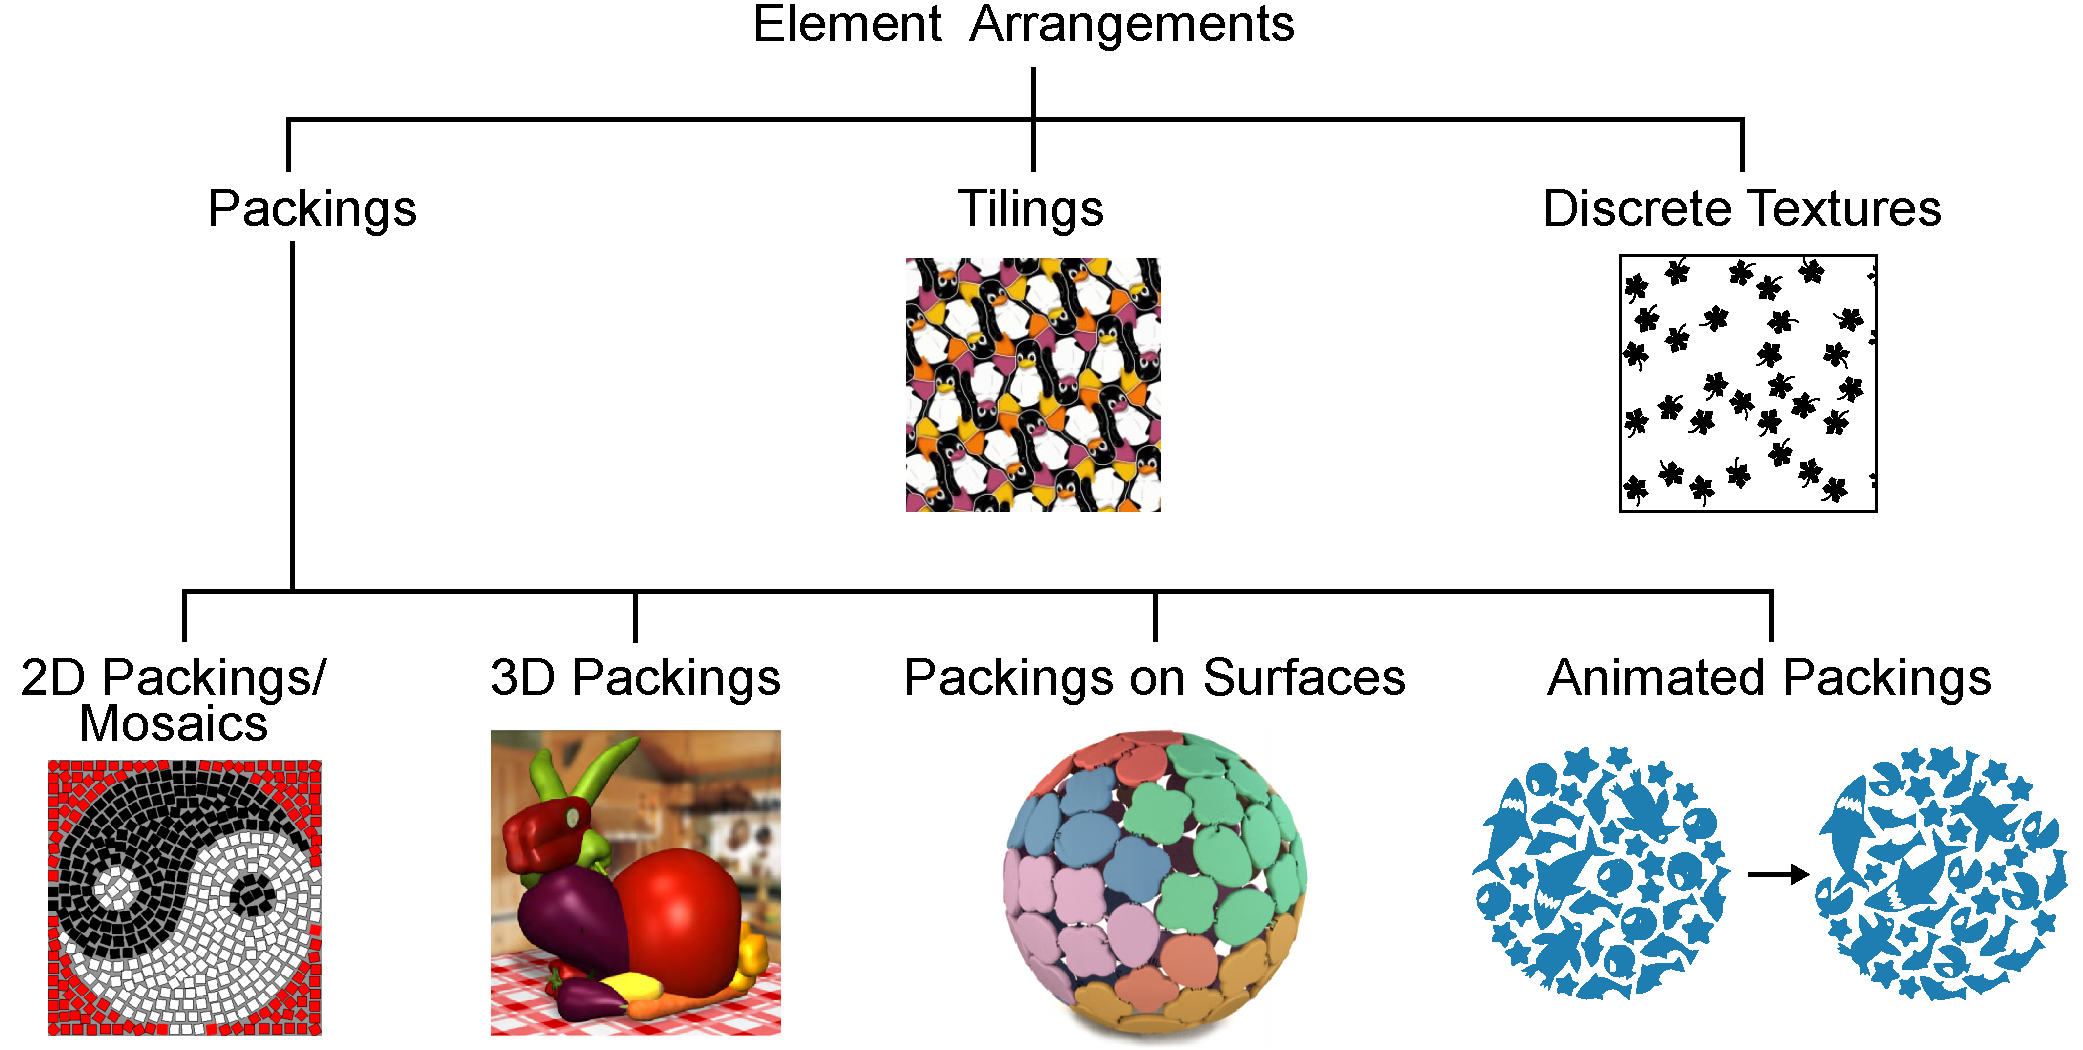
\includegraphics[width=1.0\textwidth]{figures/related/taxonomy.pdf} 
\caption[A classification of element arrangements]
{\label{fig_taxonomy} 
\nnewtext
{
A simplified classification of element arrangements.
}
}
\end{figure}


\begin{figure}
\centering
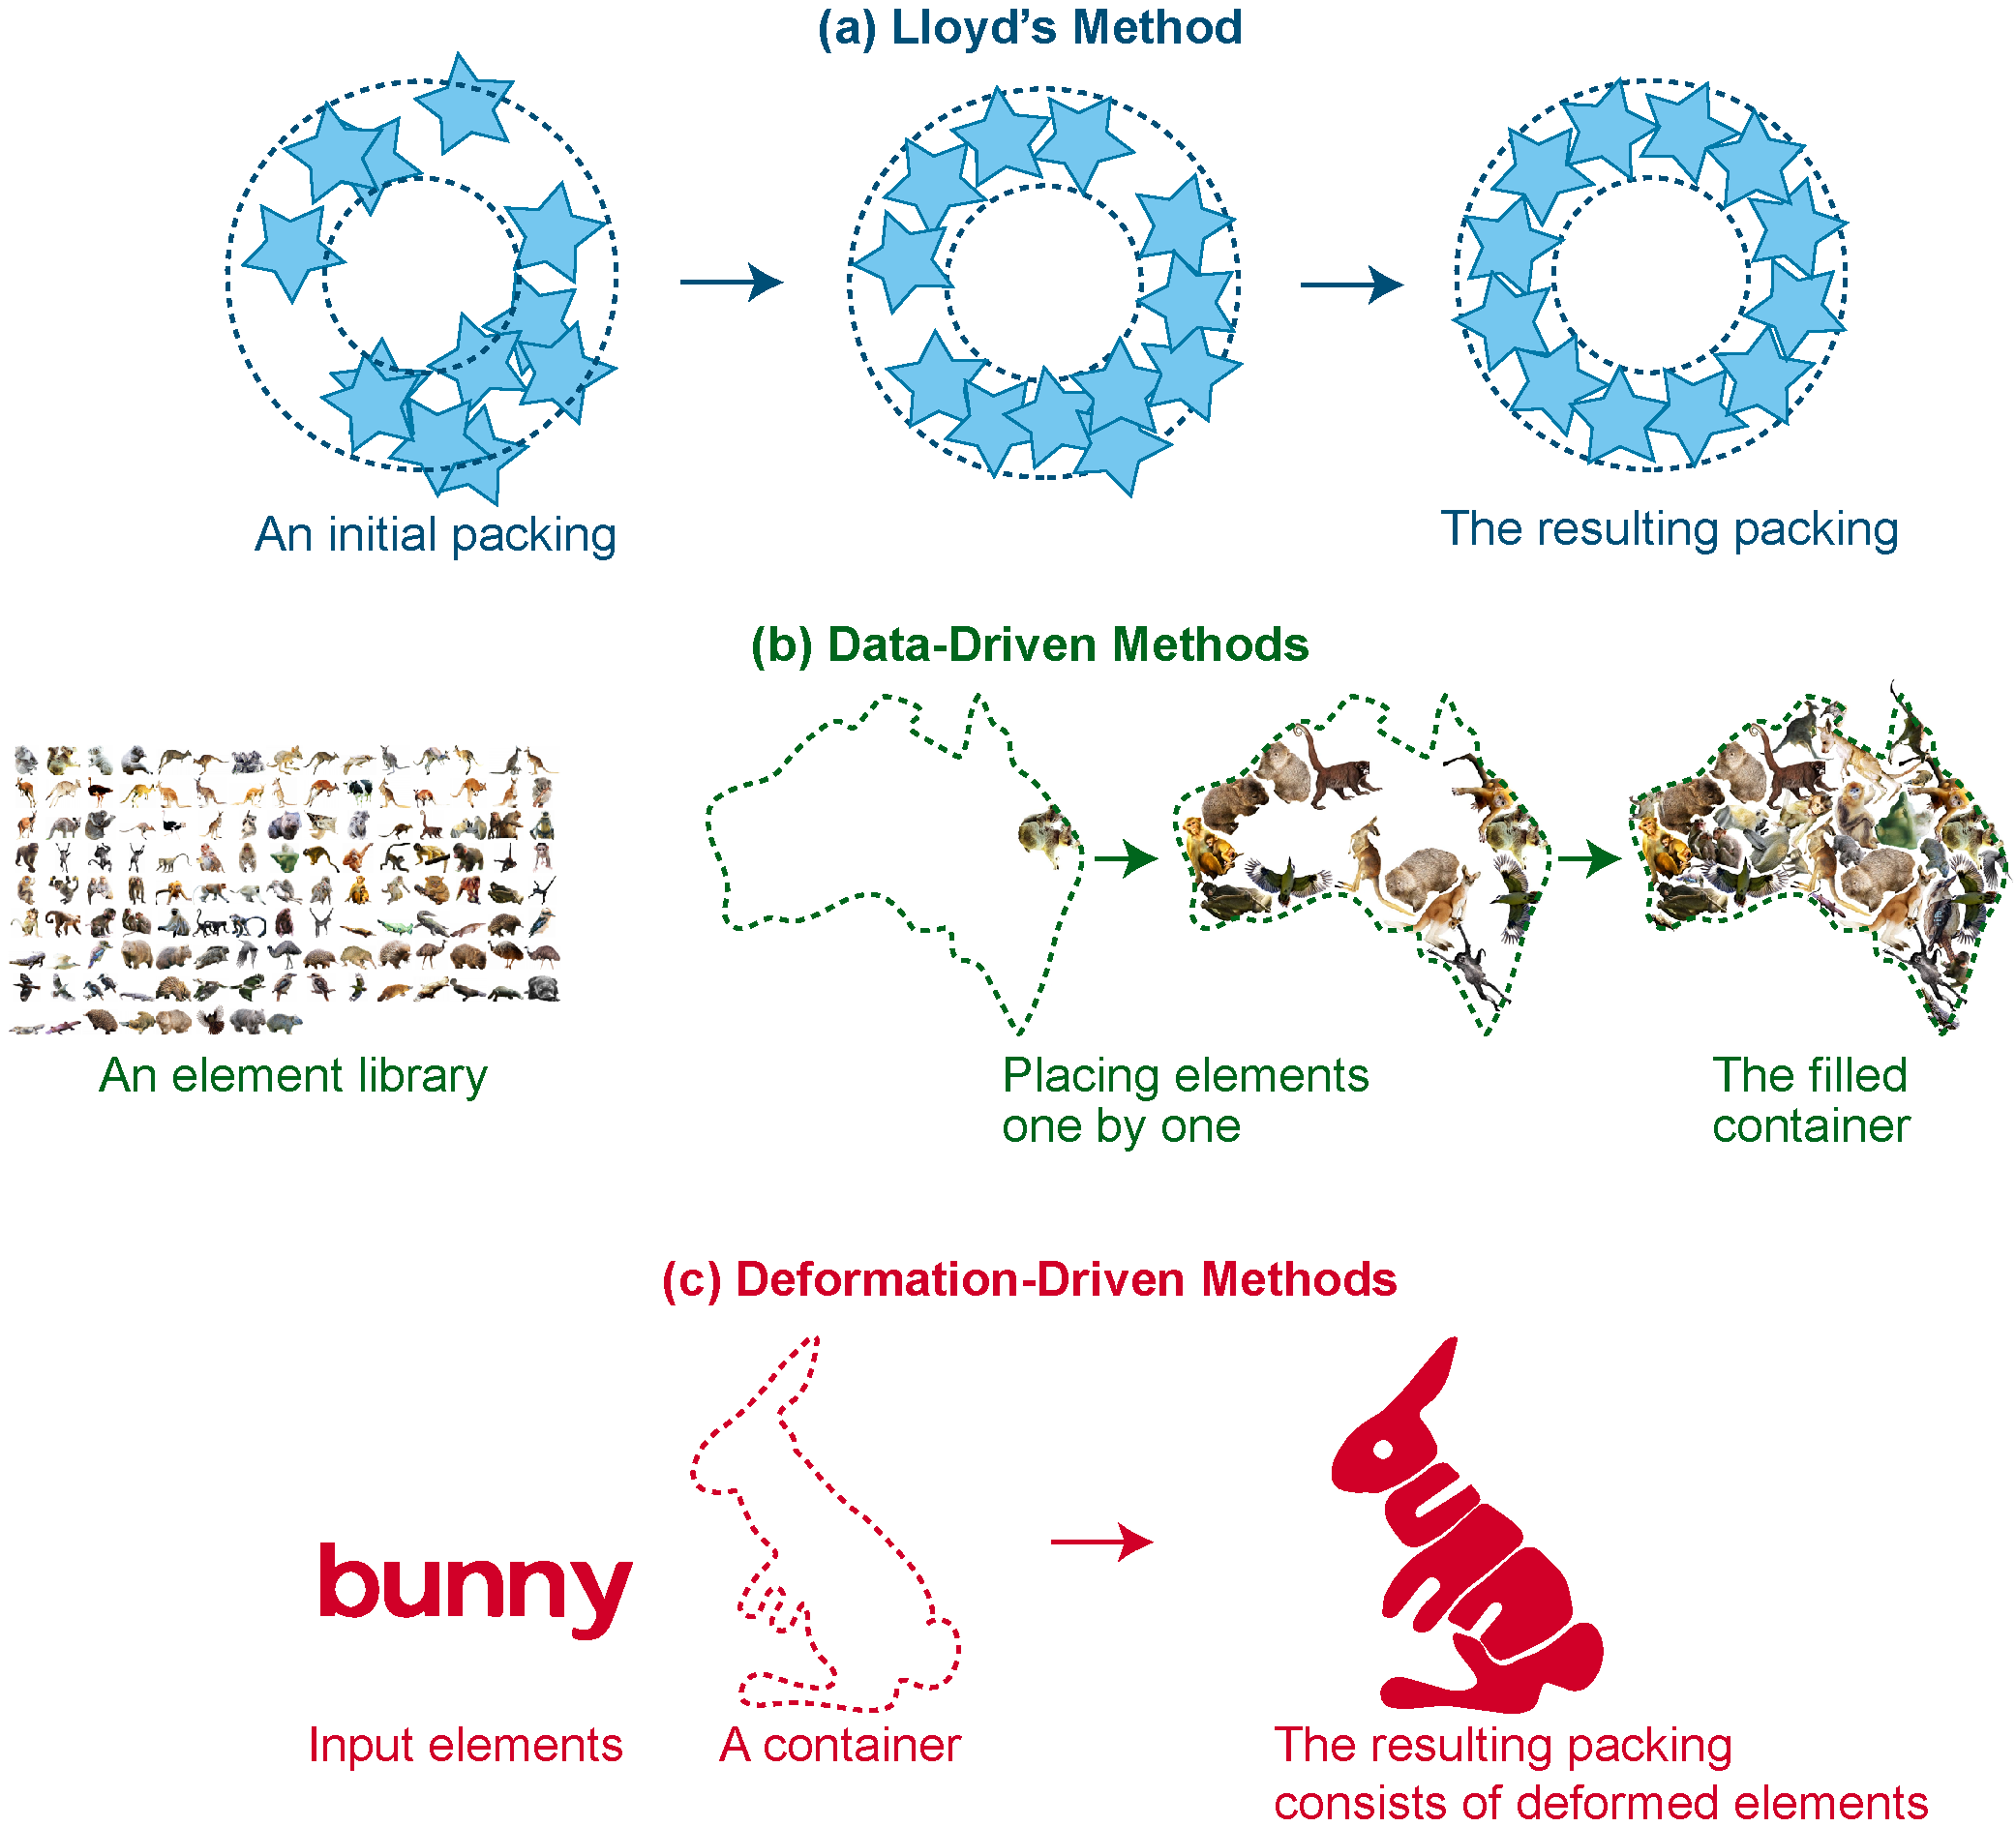
\includegraphics[width=1.0\textwidth]{figures/related/taxonomy_method.pdf} 
\caption[A classification of packing methods]
{\label{fig_taxonomy_method} 
\nnewtext
{
Popular methods in mosaicing and packings can be grouped into three categories.
%Many mosaicing and packing methods can be grouped into three categories. 
(a) Lloyd's method starts with an initial distribution of elements then iteratively distribute them
to generate a more even packing. 
(b) A data-driven method places elements one by one until the container is filled.
For each step, it select an element from an element library that is compatible with previously placed elements and the container.
(c) A deformation-driven method attempts to create element compatibility through deformation.
The illustrations are adapted from the spectral approach~\cite{Dalal2006}, 
pyramid of arclength descriptors~\cite{Kwan2016}, and
legible compact calligrams~\cite{Zou2016}
}
}
\end{figure}

\nnewtext
{
An element arrangement is defined as a distribution of non-overlapping elements in the plane.
Decades of research in NPR have produced copious amount of techniques for producing computer-generated element arrangements.
Based on their designs, categories of elements arrangements include
packings, tilings, and discrete textures (Figure~\ref{fig_taxonomy}).
The categorization can be further expanded but we only choose ones that are related to this thesis.
We further break down the packing category into several subcategories: mosaics, 2D packings, 3D packings, 
packings on surfaces, and animated packings.
This chapter covers all subcategories except animated packings that are discussed in Chapter~\ref{chapter_animationpak}. 
Many packing methods discussed in this chapter aim to minimize element overlaps, and
a few computer-generated packings shown in this chapter 
contain overlaps to some degree due to the challenge of finding and aligning compatible elements.
}

\nnewtext
{
Based on their techniques, packing methods can be grouped into three categories (Figure~\ref{fig_taxonomy_method}).
The first category, Lloyd's method, iteratively refines an initial element arrangement to generate a more even distribution.
The second category, data-driven methods, places elements one by one. For each step, a data-driven method select 
an element from an element library that is compatible with previously placed elements and the container boundary.
The last category, deformation-driven methods, attempts to create element compatibilities through shape deformation.
}

%%%%%%%%%%%%%%%%%%%%%%%%%%%%%%%%%%%%%%%%%%%%%%%%%%%%%%%%%%
\section{Mosaics}
%%%%%%%%%%%%%%%%%%%%%%%%%%%%%%%%%%%%%%%%%%%%%%%%%%%%%%%%%%
\nnewtext
{
Mosaics are 2D arrangements that are popular for decorating floors or walls.
Traditionally, elements made of stone, ceramics, or glass.
The majority of these mosaicing techniques use Llyod's method to distribute elements
via rigid transformations (Figure~\ref{fig_taxonomy_method}a).
Originally, Lloyd's method was proposed by McCool and Fiume to distribute point elements~\cite{McCool1992}.
In later work, it is generalized to distribute convex and concave elements.
}

\nnewtext
{
We first discuss the simplest variant of Lloyd's method that distributes point elements, 
as shown in Figure~\ref{fig_lloyds_method}.}
\newtext{Given $N$ point elements, we first compute a \textit{Voronoi diagram} that partitions the plane into $N$ regions such that
all points inside a Voronoi cell are closest to its associated point element.
Lloyd's method moves every point element to the centroid of its Voronoi cell, 
then the Voronoi diagram is recomputed.
The process is repeated until the distribution is even,
that means all the point elements are located at the centroids of the Voronoi cells.
The final structure is called a \textit{centroidal Voronoi diagram} (CVD).
}

\nnewtext{When computing centroids, a standard CVD assumes the area density is uniform everywhere.}
\newtext{Secord~\cite{Secord2002} computed a weighted CVD so that the resulting point element distribution
resembles a stippling artwork (Figure~\ref{fig_related_secord_hausner}a).}
\nnewtext{His method incorporates the pixel intensities of an input image as area densities. 
This alters the centroid calculation so that point elements are attracted to low-intensity regions.}

\newtext{A standard CVD is generated using Euclidean distance, but other metrics lead to different shapes of Voronoi cells.
Hausner~\cite{Hausner2001}} \nnewtext{simulated the appearance of traditional mosaics by using} 
\newtext{Manhattan distance, producing Voronoi cells that resemble squares instead of hexagons.
Each Voronoi cell is then replaced with a square element and the resulting arrangement
resembles the appearance of traditional mosaics (Figure~\ref{fig_related_secord_hausner}b). 
However, a standard CVD computes only the positions of the square elements, and Hausner must
incorporated a vector field to modify the orientation of the metric
and rotate the square elements. 
Additionally, the approach is only suitable for square elements as
more complicated shapes, such as long rectangles, would have severe overlaps.}
\nnewtext{More recently, Doyle et al.~\cite{Doyle2019} and Javid et al.~\cite{Javid2019} generated pebble mosaics 
using a superpixel image segmentation~\cite{Achanta2012}, which is a variant Lloyd's method that incorporates Euclidean metric and a CIELAB color metric.
They later elongated the Voronoi cells to follow the gradient of the input image, 
and smoothed out the cell boundaries. 
The resulting Voronoi cells resemble smooth elongated pebble shapes.
}

\begin{figure}
\centering
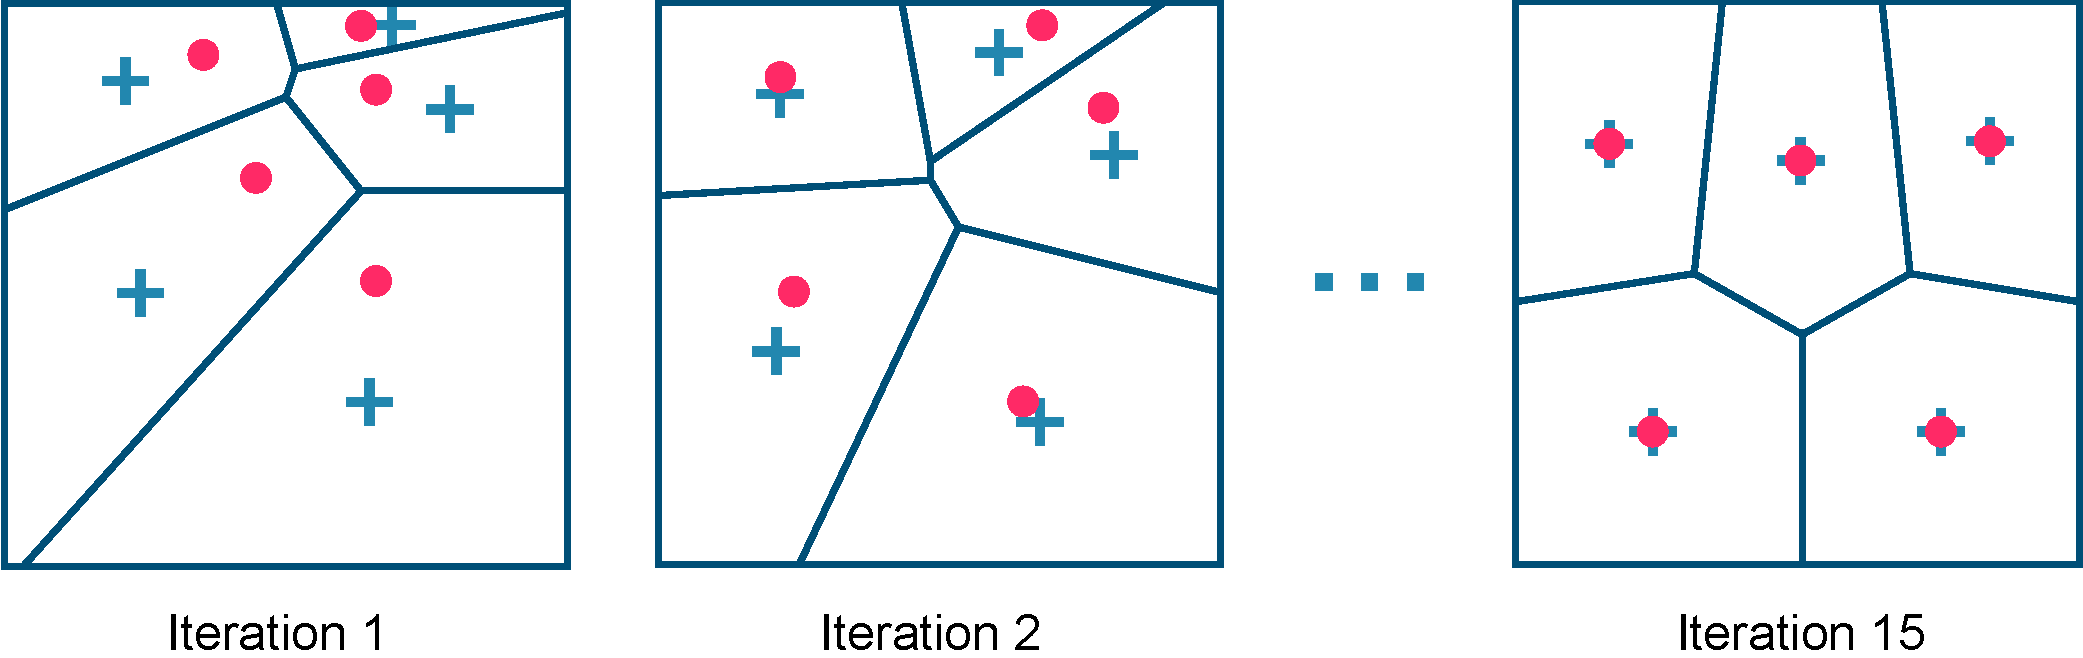
\includegraphics[width=1.0\textwidth]{figures/related/lloyds_method.pdf} 
\caption[An illustration of Lloyd's method.]
{\label{fig_lloyds_method} 
\newtext
{
An illustration of point-based Lloyd's method.
A Voronoi diagram is generated from the input point elements (drawn as red dots).
We then move the point elements to the centroids of Voronoi cells (drawn as plus signs).
The process is repeated until convergence, producing a centroidal Voronoi diagram.
Figure source is Wikipedia, drawn by Dominik Moritz under CC0 1.0.
}
}
\end{figure}


\begin{figure}
\centering
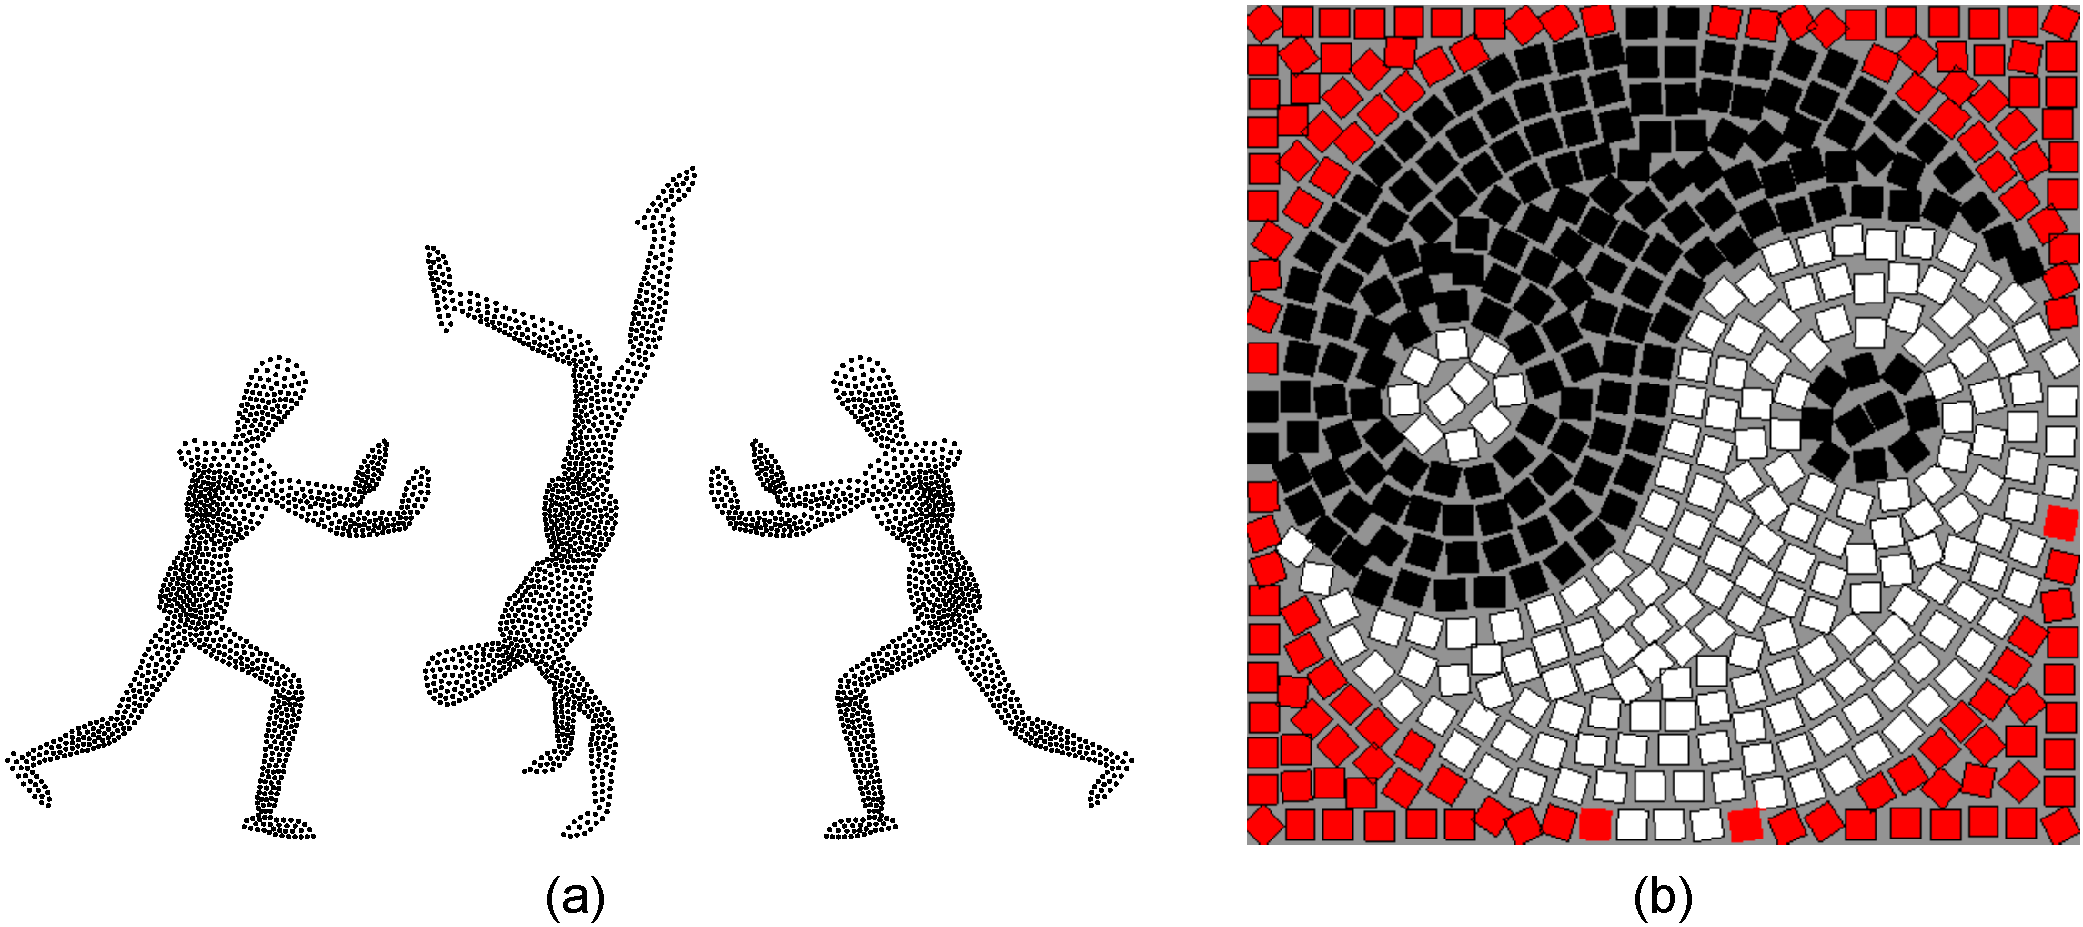
\includegraphics[width=1.0\textwidth]{figures/related/secord_hausner.pdf} 
\caption[Stippling artwork and traditional mosaics]
{\label{fig_related_secord_hausner} 
\nnewtext
{
(a) Stippling artwork of point elements generated using Lloyd's method 
that incorporates pixel densities of the input image~\cite{Secord2002}.
(b) Mosaics of square elements generated using Lloyd's method with Manhattan distance~\cite{Hausner2001}
}
}
\end{figure}

\nnewtext{We now discuss the computation of Voronoi diagrams that is generalized 
to any shapes for which a distance measurement exists.} 
\newtext
{Hiller et al.~\cite{Hiller2003} extended Lloyd's method to construct \textit{centroidal area Voronoi diagrams} (CAVDs),
a variant of CVDs that is a distribution of polygonal elements.
This new extension computes the main inertial axis for each Voronoi cell so that 
its element can be rotated to achieve better alignment with the Voronoi cell boundary.
In follow up work, Smith et al.~\cite{Smith2005} developed Animosaics to generate temporally coherent animated mosaics by utilizing CAVDs.
Dalal et al.~\cite{Dalal2006} proposed a spectral approach based on a fast Fourier transform to reposition
elements so that they achieve the best alignments with their Voronoi cell boundaries, 
which could be seen as making more effective use of negative
space, and permitting non-convex elements to interlock more than they did in
earlier methods.}
\nnewtext{However, the spectral approach cannot rotate the elements,
so it resorts to a brute force approach to find the best orientation.
Just like Animosaics, the spectral approach can generate animated mosaics,
a topic that we will explore further in Chapter~\ref{chapter_animationpak}.}

\begin{figure}
\centering
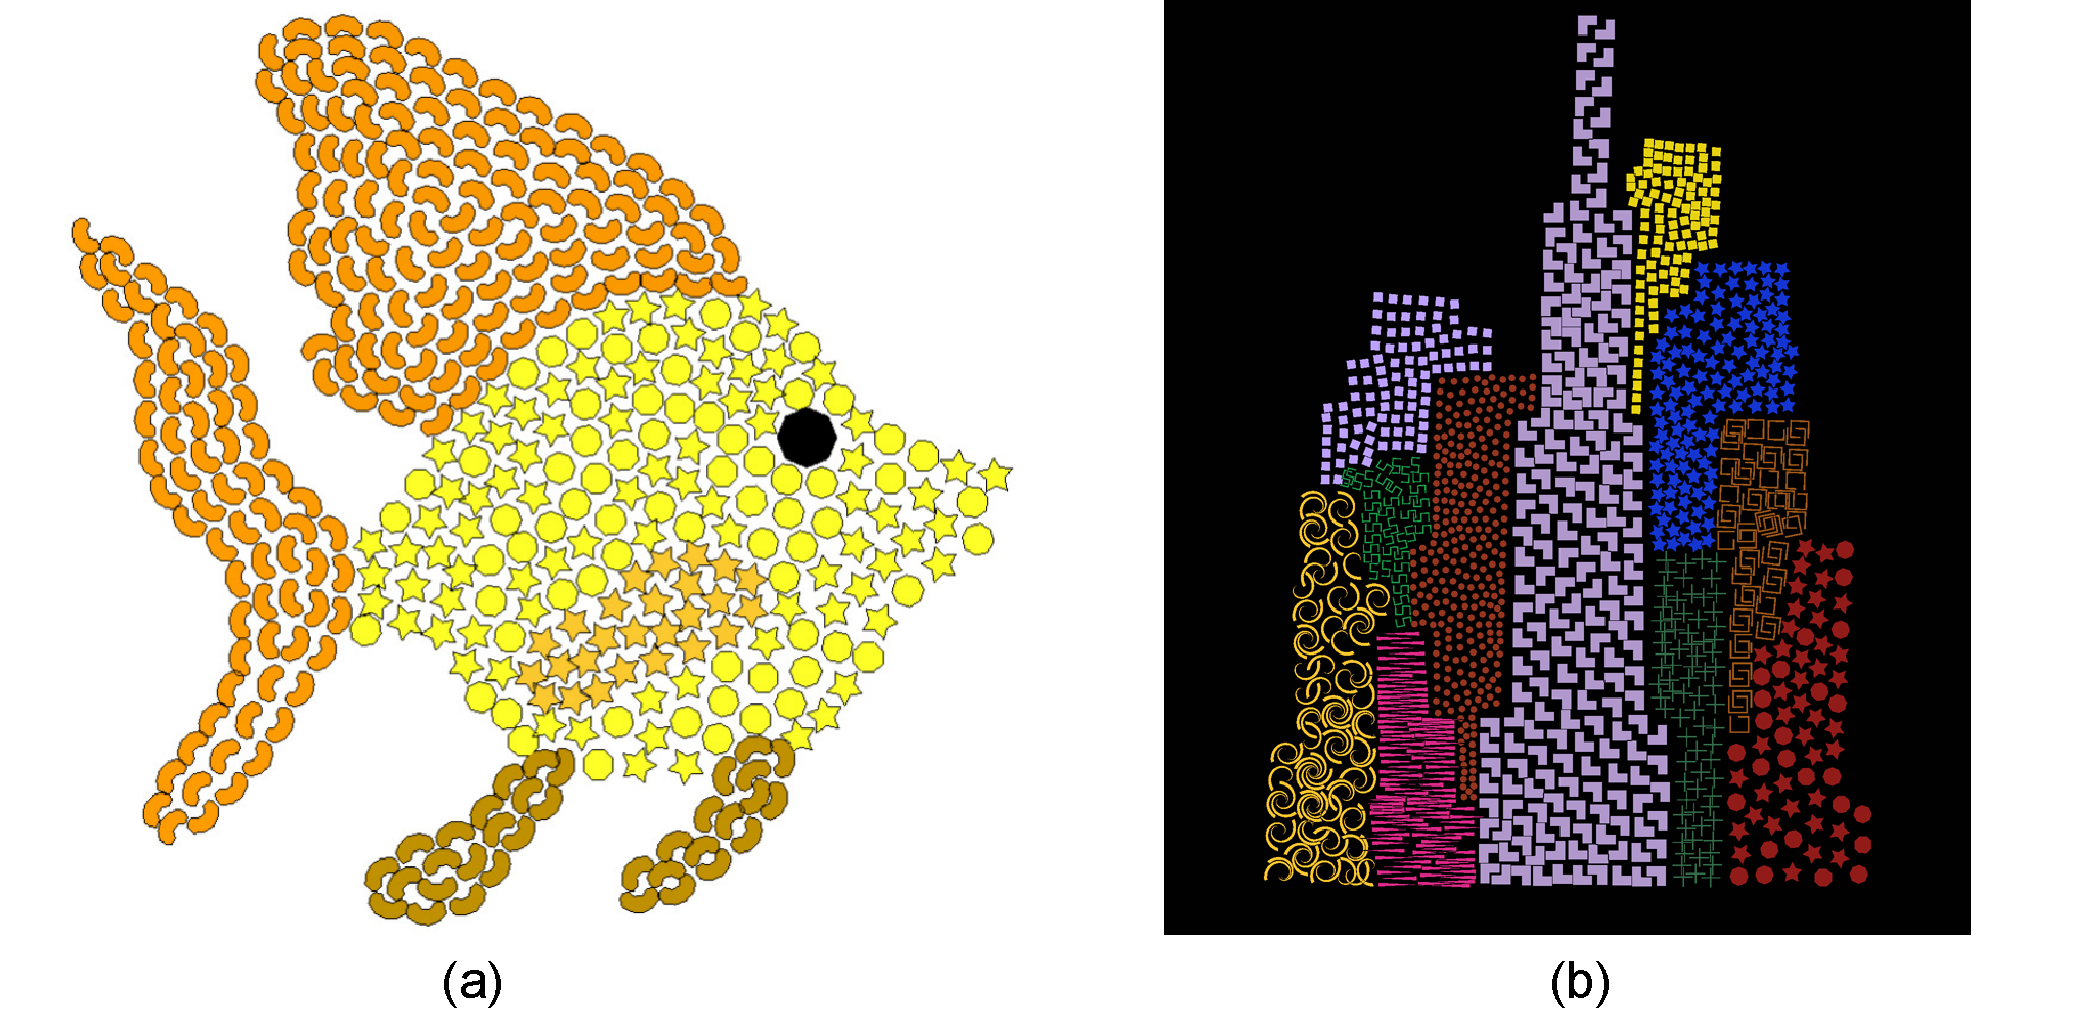
\includegraphics[width=1.0\textwidth]{figures/related/smith_dalal.pdf} 
\caption[Mosaics generated using generalized Lloyd's methods]
{\label{fig_related_secord_hausner} 
\nnewtext
{
Mosaics generated with generalized Voronoi diagrams.
(a) Animosaics~\cite{Smith2005}.
(b) A Spectral Approach~\cite{Dalal2006}.
}
}
\end{figure}

\nnewtext{As an alternative to Lloyd's method, an interactive user interface can also be used to generate mosaics.
Abdrashitov et al.~\cite{Abdrashitov2014} developed
a sketch-based interface where an artist can draw curves where square-like elements are placed along it
create a mosaic arrangement.
After the square elements are frozen in place, 
their boundaries are sliced to eliminate overlaps. }

%%%%%%%%%%%%%%%%%%%%%%%%%%%%%%%%%%%%%%%%%%%%%%%%%%%%%%%%%%
%\section{2D Mosaics and Packings}
%%%%%%%%%%%%%%%%%%%%%%%%%%%%%%%%%%%%%%%%%%%%%%%%%%%%%%%%%%

%\nnewtext
%{
%This section discusses related methods that generate 2D mosaics or packings,
%which are about arranging 2D elements tightly in a 2D container.
%Both mosaics and packings have a similar goal of creating a composition that have even distribution while minimizing overlaps.
%A packing with an even distribution has its positive and negative space approximately uniform.
%The gaps between elements should roughly have the same width.
%Visually, traditional mosaics often use near convex elements made of stone, ceramics, or glass,
%while 2D packings are composed of elements that have more general 
%shapes that are either convex or concave.
%}

%\nnewtext{
%An approach to generate a packing is to start with an initial configuration and 
%iteratively refine it using \textit{Lloyd's method}~\cite{McCool1992}.}
%\newtext{
%Figure~\ref{fig_lloyds_method} shows an illustration of point-based Lloyd's method.
%Given $N$ point elements, 
%we first compute a \textit{Voronoi diagram} that partitions the plane into $N$ regions such that
%all points inside a Voronoi cell are closest to its associated point element.
%Lloyd's method moves every point element to the centroid of its Voronoi cell, 
%then the Voronoi diagram is recomputed.
%The process is repeated until the distribution is even,
%that means all the point elements are located at the centroids of the Voronoi cells.
%The final structure is called a \textit{centroidal Voronoi diagram} (CVD).
%}

%\newtext
%{
%A standard CVD is generated using Euclidean distance metric, but it can be replaced
%to manipulate the shapes of Voronoi cells.
%Hausner~\cite{Hausner2001} used this idea to distribute square elements into a container 
%region, simulating the appearance of traditional mosaics (Figure~\ref{fig_related_hausner}). 
%This can be achieved by using Manhattan distance metric so that Voronoi cells resemble squares instead of hexagons.
%This approach can only position the square elements to be centered at the Voronoi centroids, and it must
%incorporate a vector field to modify the orientation of the metric
%and rotate the square elements. 
%In conclusion, Hausner's approach is only suitable for square elements as
%more complicated shapes such as long rectangles would have severe overlaps.
%More recently, Javid et al.~\cite{Javid2019} constructed a metric that 
%incorporates a spatial distance, a color distance, and an elongation factor. Their resulting
%Voronoi cells have elongated shapes, resembling pebble-like mosaics.}

\section{2D Packings}

\nnewtext
{
This section discusses packing methods that fall into the categories of data-driven ((Figure~\ref{fig_taxonomy_method})b) and 
deformation-driven (Figure~\ref{fig_taxonomy_method}c).
Unlike mosaics, these packings are composed of 
more intricate elements that resemble man-made objects, plants, or animals.
Additionally, some packing styles are reminiscent to Giuseppe Arcimboldo's paintings 
(Figure ~\ref{fig_related_arcimboldo}).}


\nnewtext
{
A data-driven method requires an input element library to find compatible elements (Figure~\ref{fig_related_jim_pad}).}
\newtext{This is usually done by placing elements one by one until the container area is filled.
A shape matching algorithm selects an 
element from the library that has the best compatibility with the previously placed elements or the container boundary.
Jigsaw Image Mosaics~\cite{Kim2002} uses a geometric hashing technique to find
compatible elements. JIM method places elements using a greedy approach, but is able to backtrack 
if a previous configuration is more optimal.
Pyramid of Arclength Descriptor (PAD)~\cite{Kwan2016} is a curvature-based shape descriptor that
can find new elements that partially match
existing element boundaries as a container was being filled. }


\newtext{\nnewtext{An alternative approach to data-driven methods} is to initially partition a container into smaller segments
then independently replace each segment with a matching element \nnewtext{taken from the library}.
This is desirable if the container has colors or salient parts that need to be emphasized.
Huang et al.~\cite{Huang2011} proposed a data-driven approach that generates Arcimboldo-like collages
by arranging cutout images collected from the internet.
Their container is a larger cutout image which is partitioned into parts
using an image segmentation algorithm.
Each part is then replaced with a smaller cutout image that has a similar shape and color.
}

\newtext
{
All these data-driven methods require a large element library.
The more elements in the library, the better the chances of finding compatible elements.}
\nnewtext
{
For example, JIM method required about 900 elements, PAD used a library with more than 120 elements 
(see Figure~\ref{fig_taxonomy_method}), 
and Huang et al. needed about 5000 elements.}
\newtext
{However, a bigger database means increased computational time and
collecting a large number of elements is not always feasible.}

\nnewtext{ 
After the container is filled, these data-driven methods permit some elements to overlaps,
which are later corrected using deformation.
This is a post-processing step where the elements are frozen in place and
the deformation is applied locally near element boundaries.
The use of deformation can be interpreted as improving the element compatibilities, 
but only locally as these methods still need a large element library to generate satisfactory packings.} 
%This deformation step later is further exploited by deformation-driven methods.

\begin{figure}
\centering
\includegraphics[width=1.0\textwidth]{figures/related/arcimboldo.pdf} 
\caption[Vertumnus painting by Giuseppe Arcimboldo]
{\label{fig_related_arcimboldo} 
\nnewtext
{
Vertumnus painting by Giuseppe Arcimboldo that illustrates
a packing of plants, vegetables, and fruits
(Skokloster Castle, Skokloster, Sweden). 
}
}
\end{figure}

\begin{figure}
\centering
\includegraphics[width=1.0\textwidth]{figures/related/jim_pad.pdf} 
\caption[Packings generated by JIM and PAD]
{\label{fig_related_jim_pad} 
\newtext
{
Data-driven methods:
(a) Jigsaw Image Mosaics~\cite{Kim2002}.
(b) Pyramid of Arclength Descriptor~\cite{Kwan2016}. 
}
}
\end{figure}




\begin{figure}
\centering
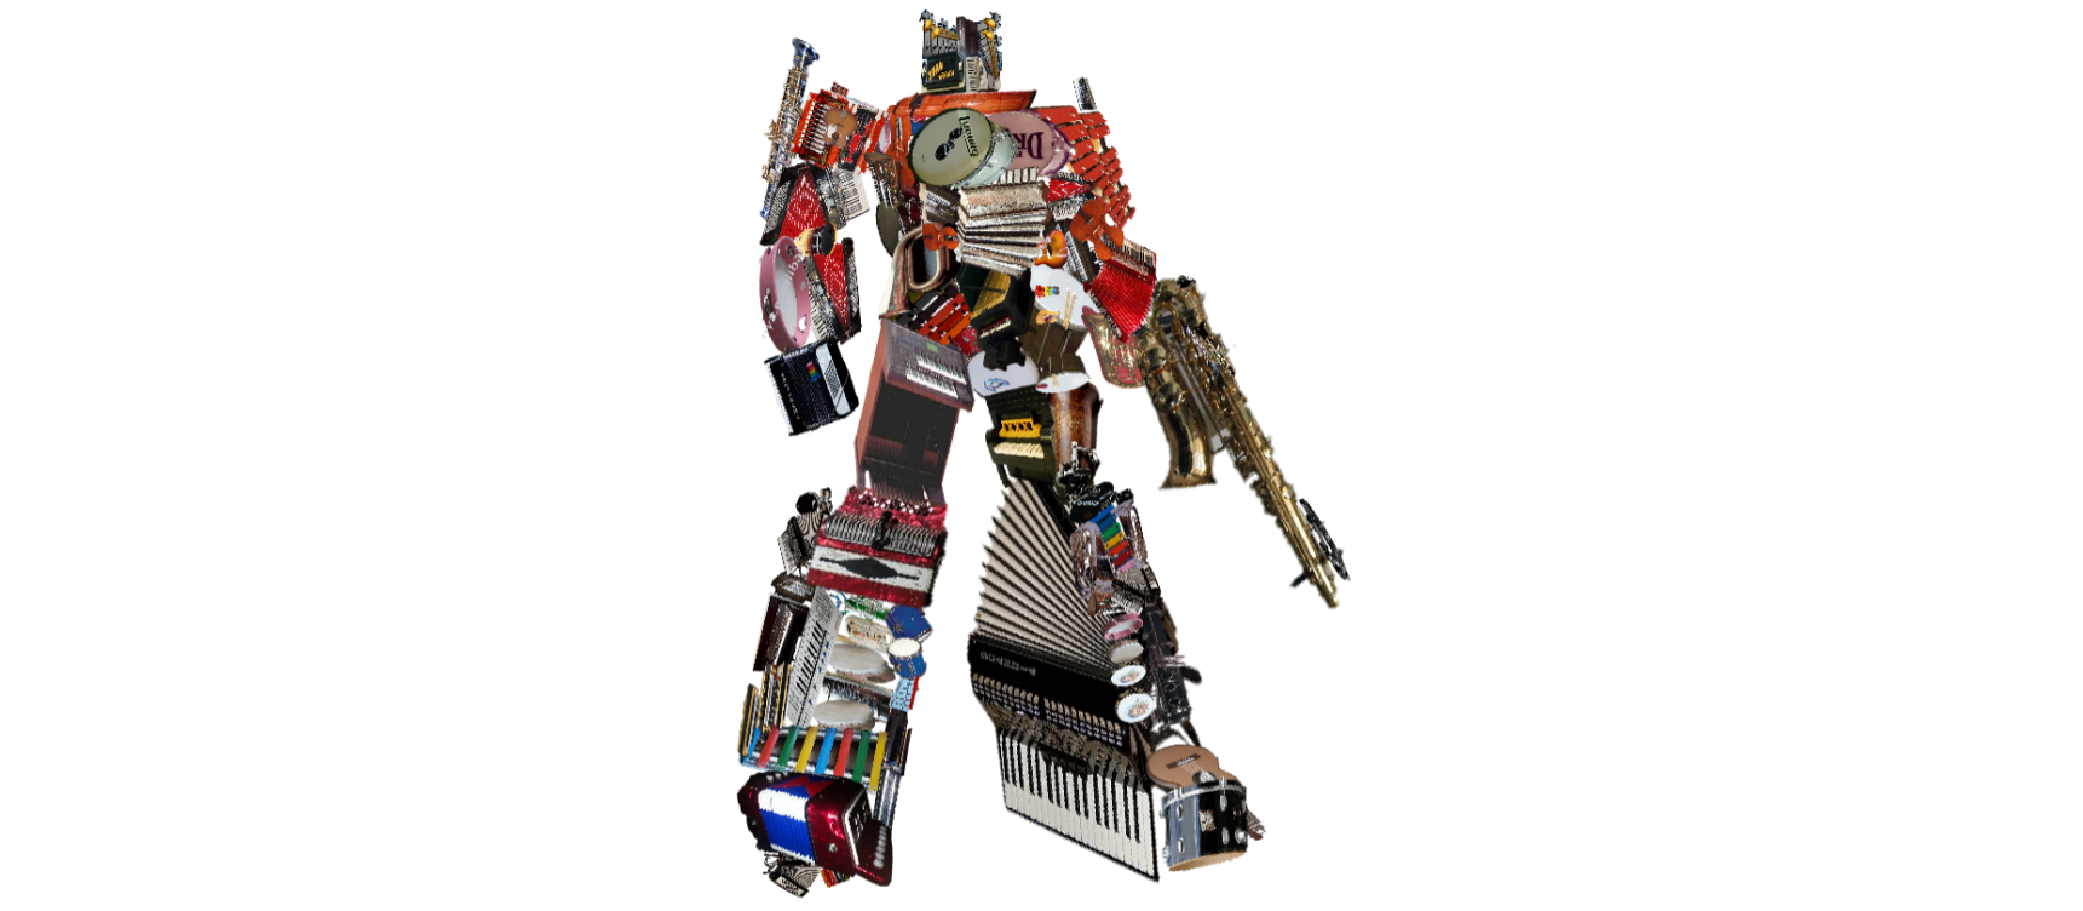
\includegraphics[width=1.0\textwidth]{figures/related/optimus.pdf} 
\caption[An Arcimboldo-inspired 2D packing]
{\label{fig_related_optimus} 
\nnewtext
{
An Arcimboldo-inspired 2D packing consisting of overlapping elements~\cite{Huang2011} .
}
}
\end{figure}

\nnewtext
{
Instead of allowing shape compatibilities to arise organically in a large collection of elements, 
we can deform elements to manufacture those compatibilities.
A deformation-driven method can create packings based on much smaller element libraries.
Xu and Kaplan~\cite{Xu2007} and Zou et al.~\cite{Zou2016} constructed calligraphic packings by filling a container with a small
number of letter elements composing one or two words (Figure~\ref{fig_taxonomy_method}c and ~\ref{fig_calligraphy_packing}a). 
Xu and Kaplan's method is able to fill the container but they shuffled the letter ordering that made it difficult to read.
The improved method by Zou et al. can achieve a better the readability by computing
the medial axis of the container where letter elements are anchored.
However, these calligraphic packing methods require significant deformation 
so they are not able to preserve the typefaces of the letters.
In another topic, Peng et al.~\cite{Peng2014} proposed a method that packs and deforms
simple polygon and polyomino elements to generate layouts for urban planning or indoor space, 
although their method cannot handle more complicated shapes. 
An example of their generated indoor layout is seen in Figure~\ref{fig_office}.
These data-driven methods were developed for specific designs: calligraphies of letterforms and urban layouts of rectangular shapes.
We see an opportunity to use deformation-driven approach to generate packings with more general styles composed
of nature or everyday objects similar to JIMs or PAD packings.
}


\begin{figure}
\centering

\includegraphics[width=1.0\textwidth]{figures/related/calligraphy.pdf} 
\caption[A calligraphy packing of an ``elephant'']
{\label{fig_calligraphy_packing} 
\newtext
{
A deformation-driven packing of a calligraphic ``elephant''~\cite{Xu2007}.
}
}
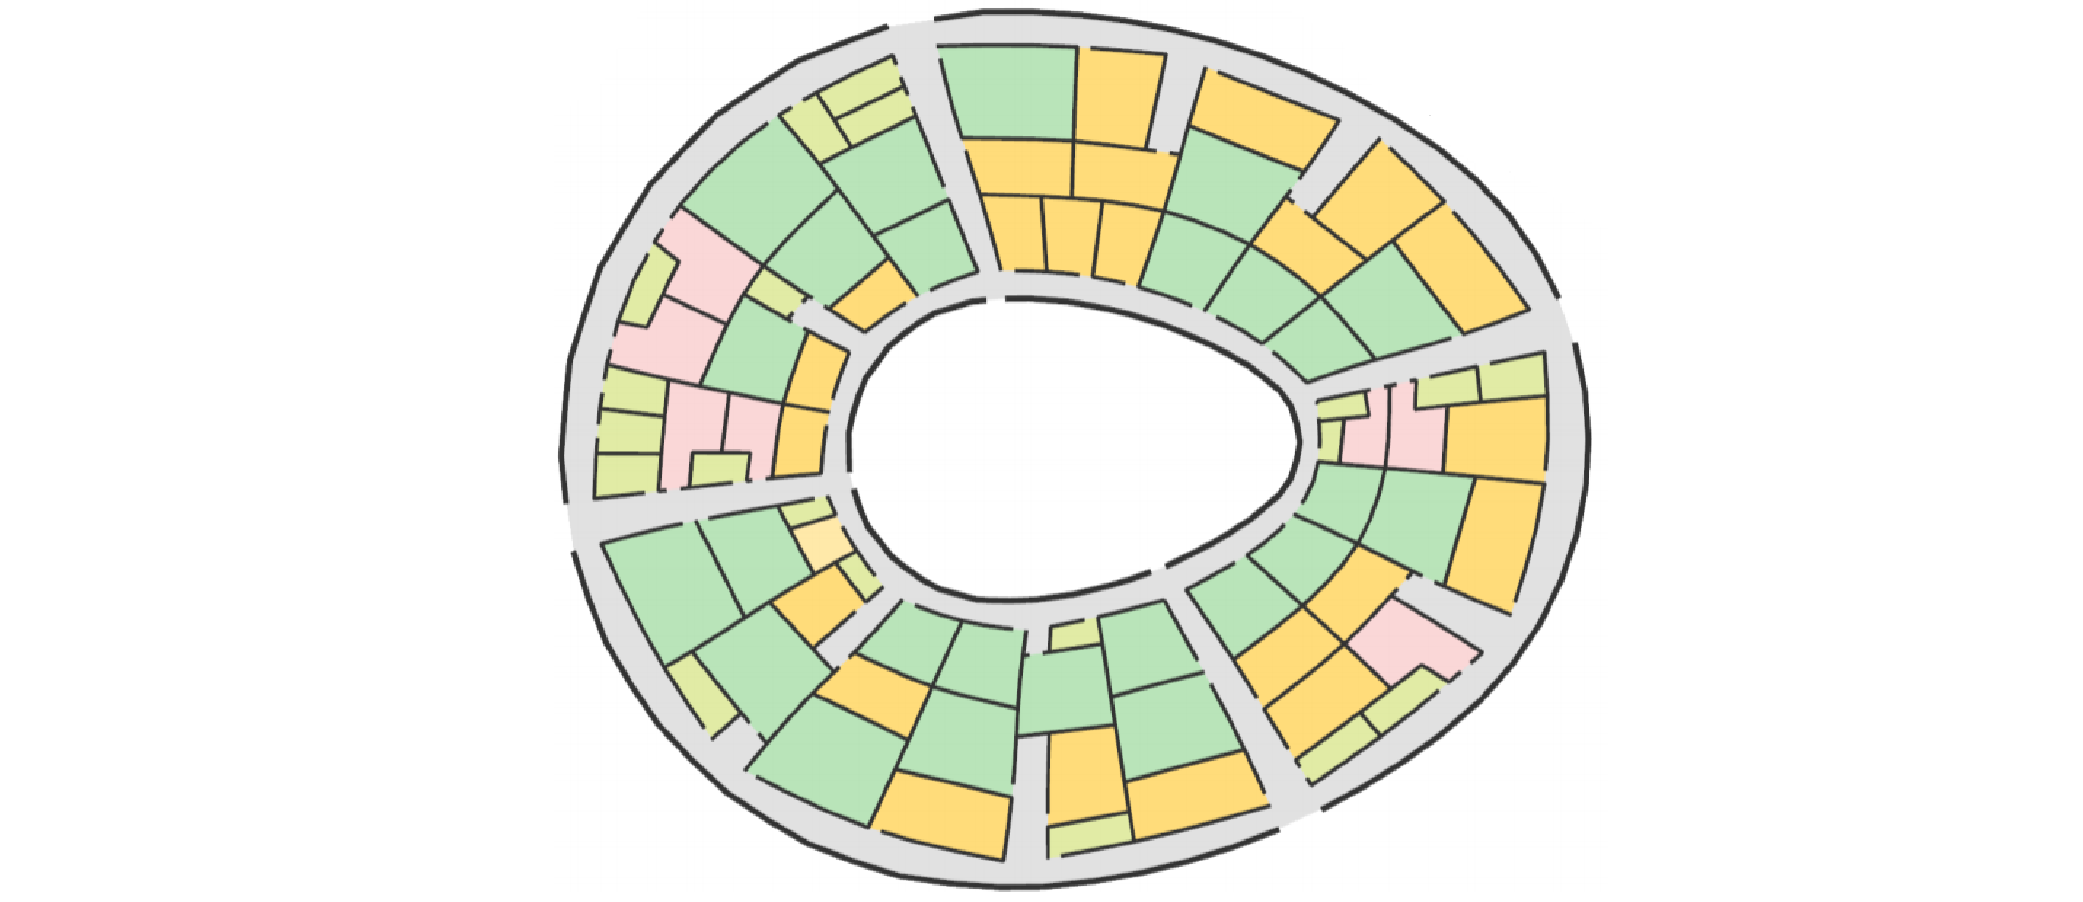
\includegraphics[width=1.0\textwidth]{figures/related/layout.pdf} 
\caption[An office layout generated by packing \newline deformable rectangle and polyomino elements]
{\label{fig_office}
\nnewtext
{
An office layout generated by packing deformable rectangle and polyomino elements~\cite{Peng2014}.
}
}
\end{figure}




%%%%%%%%%%%%%%%%%%%%%%%%%%%%%%%%%%%%%%%%%%%%%%%%%%%%%%%%%%
\section{Tilings}
\label{related_wrok_tiling}
%%%%%%%%%%%%%%%%%%%%%%%%%%%%%%%%%%%%%%%%%%%%%%%%%%%%%%%%%%

\newtext
{
As elements reach perfect compatibility, a packing turns to a tiling, as seen from an example in Figure~\ref{fig_related_escherization}.
The element boundaries interlock, leaving no negative space.
Kaplan and Salesin~\cite{Kaplan2000, Kaplan2004} deformed one or two 
input elements into shapes that can tile the plane.
The tiles always fill the entire plane, and are not intended for filling a bounded container.}
\nnewtext{Given an input element $E$, they performed a search in a parameterized tiling space to find its
deformed variant $T$.
Due to deformation,}
\newtext{$T$ is often perceptually unrecognizable from its silhouette unless an interior picture is added.}
\nnewtext{
Kaplan and Salesin's method has a better chance to find $T$ if $E$ has shallow concavities.
More recent methods~\cite{Koizumi2011, Nagata2020} are able to solve the Escherization problem more efficiently and can deal with shapes that have deeper concavities.}


%Given an input element $E$ they look for a similar tileable element $T$
%in a parameterized tiling space using simulated annealing.
%The original heuristic method has a better chance to find $T$ if $E$ has less concavity, but more recent methods
%are able to tile shapes 
%The original heuristic method can only deal withfail to find $T$ if $E$ has deep concavity, for example, a ``G'' shape.
%However, more recent methods are able to deal with this issue.

\nnewtext
{
Past research has proposed methods
to replicate the figure-ground reversal style of Escher's Sky and Water,
in which elements serve as both positive and negative space depending 
on the viewer's perception~\cite{Kaplan2004, Sugihara2009, Lin2018} .
Given two elements $S_1$ and $S_2$, each is placed on opposite sides of a rectangular canvas.
They are then copied, arranged, and deformed to interlock each other.
The farther a copy from the original element, the more deformed it is, 
creating a ``fading effect'', $S_1$ and $S_2$ spatially evolve to become negative space.
The idea of element evolutions also presents in metamorphosis tiling style,
in which interlocking elements evolve from one shape to another,
which can be interpreted as ``spatial animation''.
Kaplan~\cite{Kaplan2010} proposed several element evolution schemes to generate metamorphosis tilings:
a grid-based curve evolution, iterated function systems, and organic labyrinthine simulations.
}

\begin{figure}
\centering
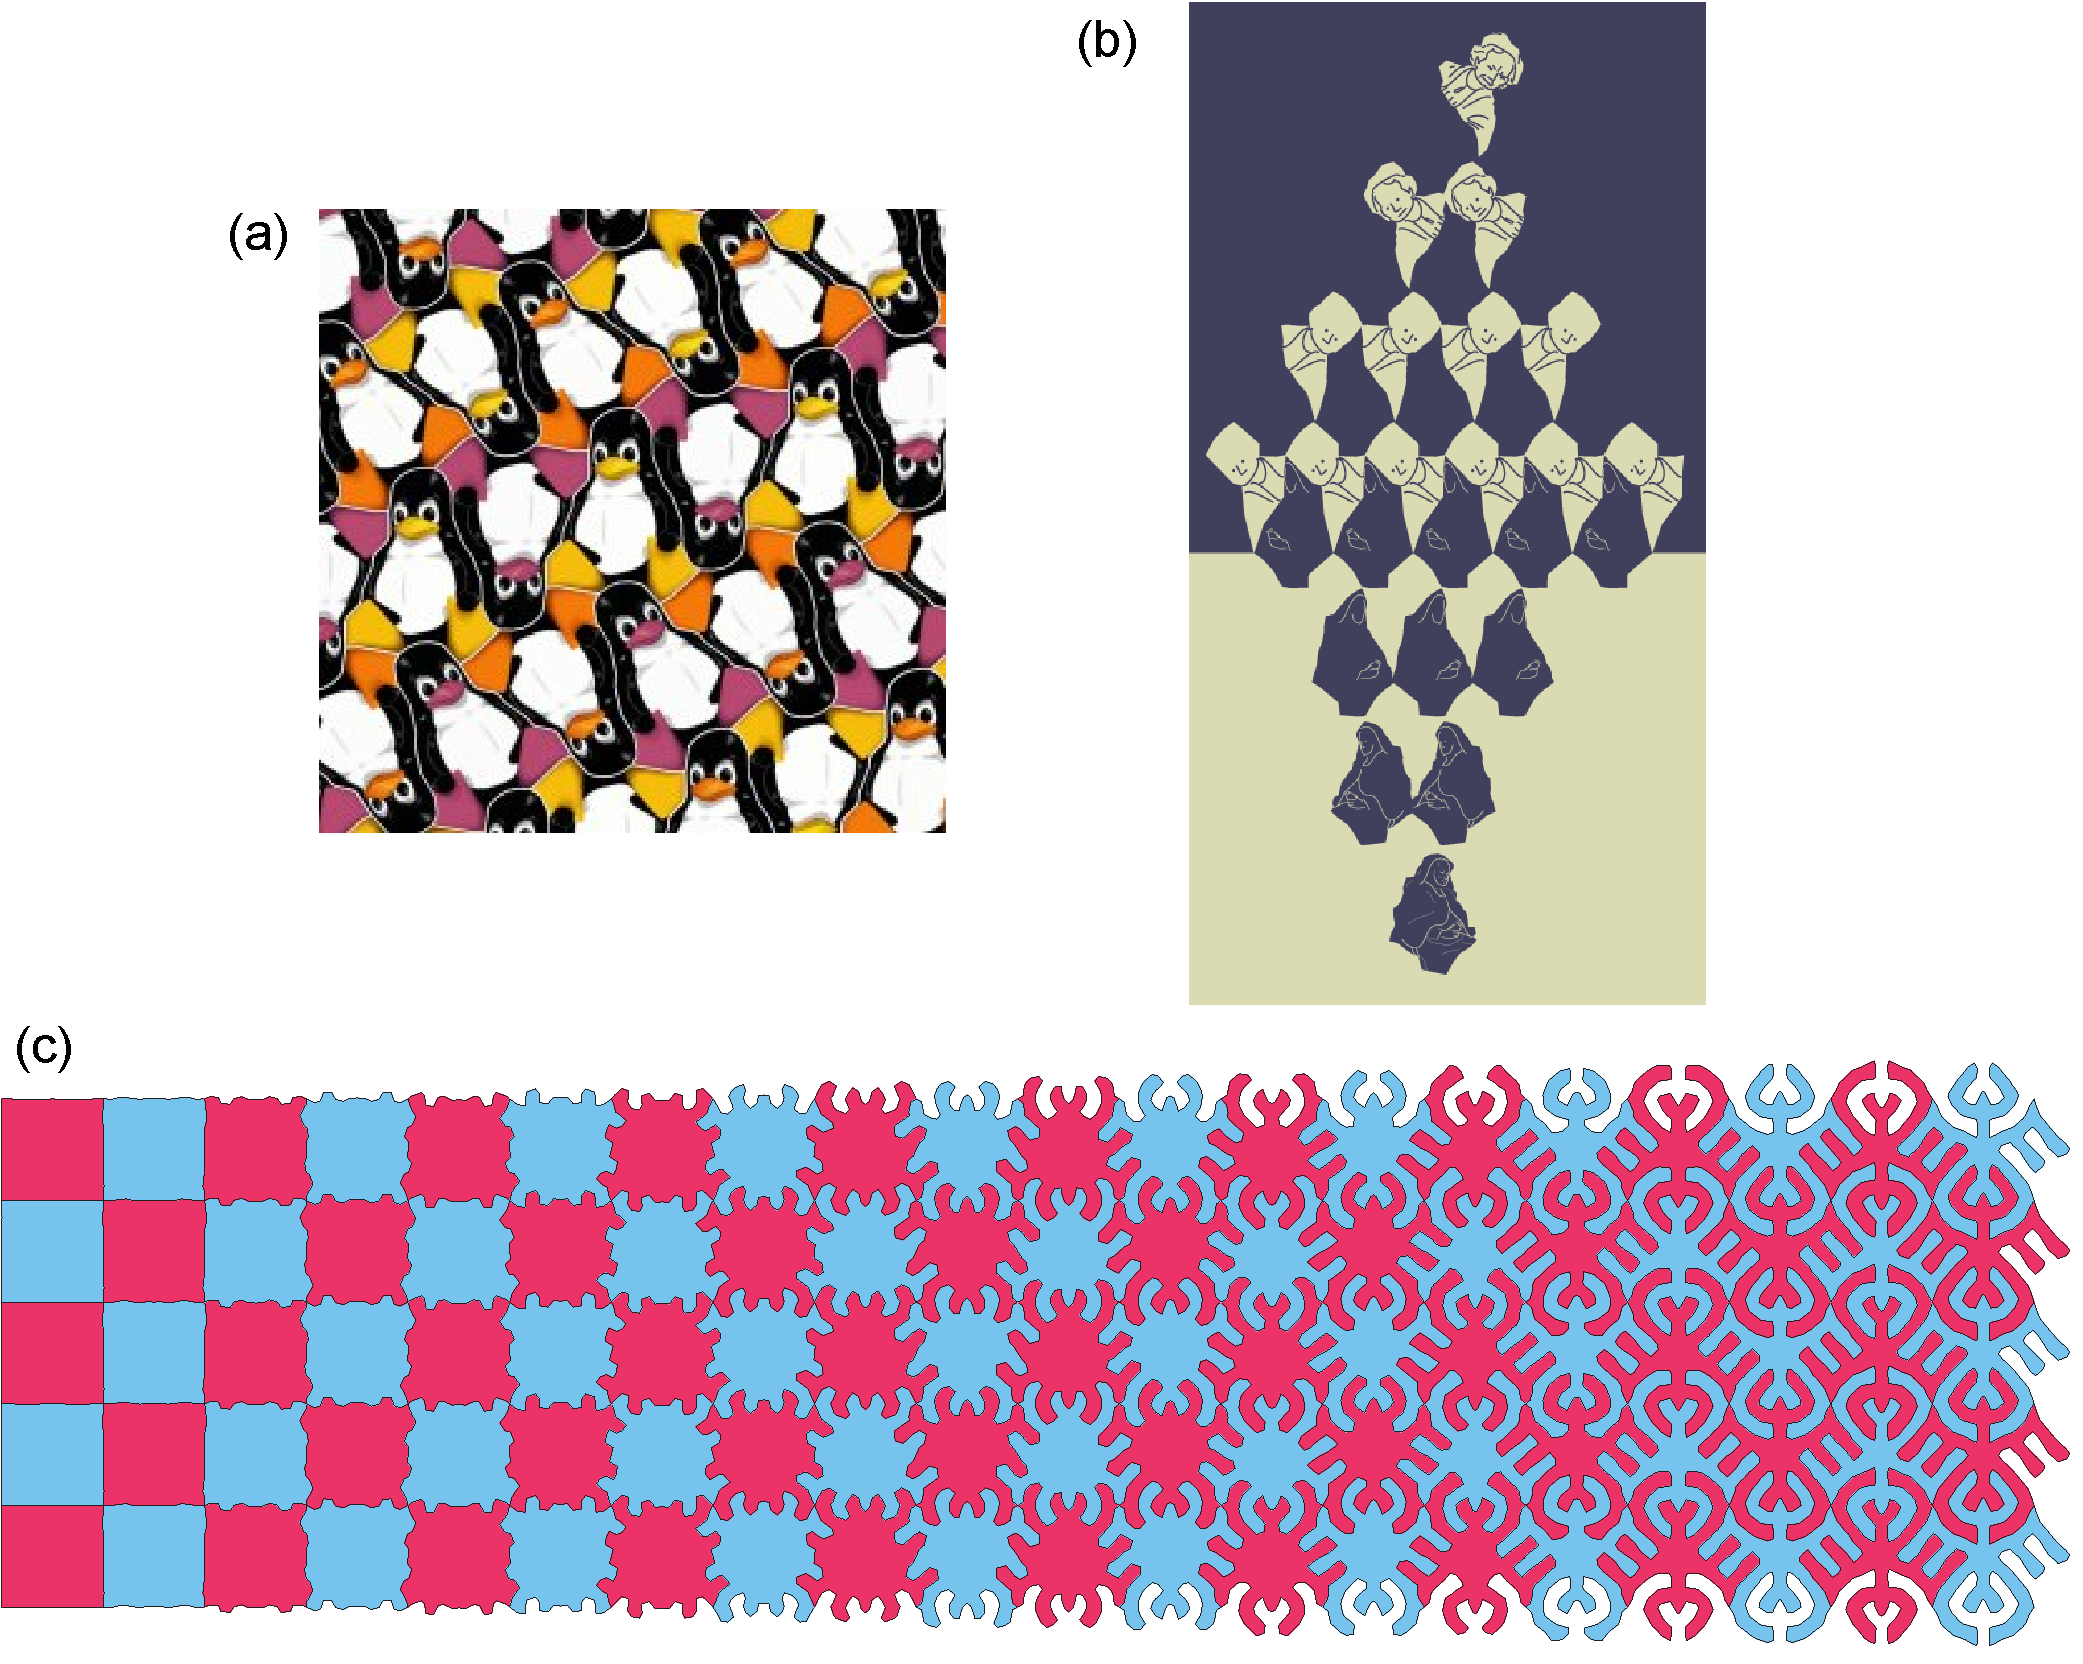
\includegraphics[width=1.0\textwidth]{figures/related/tilings.pdf} 
\caption[Tilings]
{\label{fig_related_escherization} 
\newtext
{
(a) A tiling of tux penguins~\cite{Kaplan2000}.
(b) Sky and water tiling style~\cite{Kaplan2004}.
(c) Metamorphosis tiling style~\cite{Kaplan2010}.
}
}
\end{figure}

%Given two elements $S_1$ and $S_2$, each is placed on the opposite side of a rectangular canvas.
%They are then copied, arranged, and deformed to interlock each other.
%The farther a copy from the original element, the more deformed it is and the


%\newtext
%{
%Lin et al.~\cite{Lin2018} generated ground-reversal compositions that resemble Escher's Sky and Water I,
%where elements serve as both positive and negative space depending on the viewer's perception.
%Given two elements $S_1$ and $S_2$, each is placed on the opposite side of a rectangular canvas.
%They are then copied, arranged, and deformed to interlock each other.
%The farther a copy from the original element, the more deformed it is, 
%creating a ``fading effect'', $S_1$ and $S_2$ spatially fade to nothingness.
%This work is data-driven, the user needs to provide $S_1$, 
%and the method tries to find a compatible element $S_2$ from a library.
%}





%%%%%%%%%%%%%%%%%%%%%%%%%%%%%%%%%%%%%%%%%%%%%%%%%%%%%%%%%%
\section{Discrete Texture Synthesis}
%%%%%%%%%%%%%%%%%%%%%%%%%%%%%%%%%%%%%%%%%%%%%%%%%%%%%%%%%%

\newtext
{
Some past work has sought to adapt example-based texture synthesis methods
from raster images to vector graphics, producing distributions of
rigidly transformed elements that mimic the statistics of an \textit{exemplar}, 
an example can be seen in Figure~\ref{fig_discrete_texture}.}
\nnewtext{These techniques are all concerned with replicating
the distribution of positive space in the exemplar, and less about negative space.}
\newtext{An element is represented as a single point, which is adequate for small near-convex elements.
Barla et al.~\cite{Barla2006} and Ijiri et al.~\cite{Ijiri2008} used a growth model that copies small neighborhoods
from the exemplar into a larger output texture.  
Hurtut et al.~\cite{Hurtut2009} developed a statistical sampling method based
on multitype point processes.  
AlMeraj et al.~\cite{AlMeraj2013}
stamped out copies of the exemplar and discarded overlapping elements.
Loi et al.~\cite{Loi2017} developed a texture synthesis method that
can specify global arrangements, local arrangements, or a blend of multiple arrangements.
}

\newtext
{
For larger concave elements, a single point representation is not enough.
Ma et al. ~\cite{Ma2011} used a sample-based representation that
is created by generating a sparse set of points inside an element.
They later distributed these points using a neighborhood metric and an iterative optimization.
Unlike previous work, they were able synthesize textures with long deformable elements, for example, spaghetti.
Ma et al. later extended their work to accept animated elements~\cite{Ma2013}, where
each sample point has a spatial and time position, turning the problem to spacetime texture synthesis.
More recently, Hsu et al.~\cite{Hsu2020} adapted the sample-based representation into an interactive tool
where an artist can initially distribute elements by drawing strokes
which are then optimized using a Lloyd-like optimization.
}
%Most discrete texture synthesis method treat a single element
%Ma et al.~\cite{Ma2011} used sample-based element representation 
%Ma et al.~\cite{Ma2011} use sparse point samples to represent an element, which
%give an advantage of distributing 


\begin{figure}
\centering
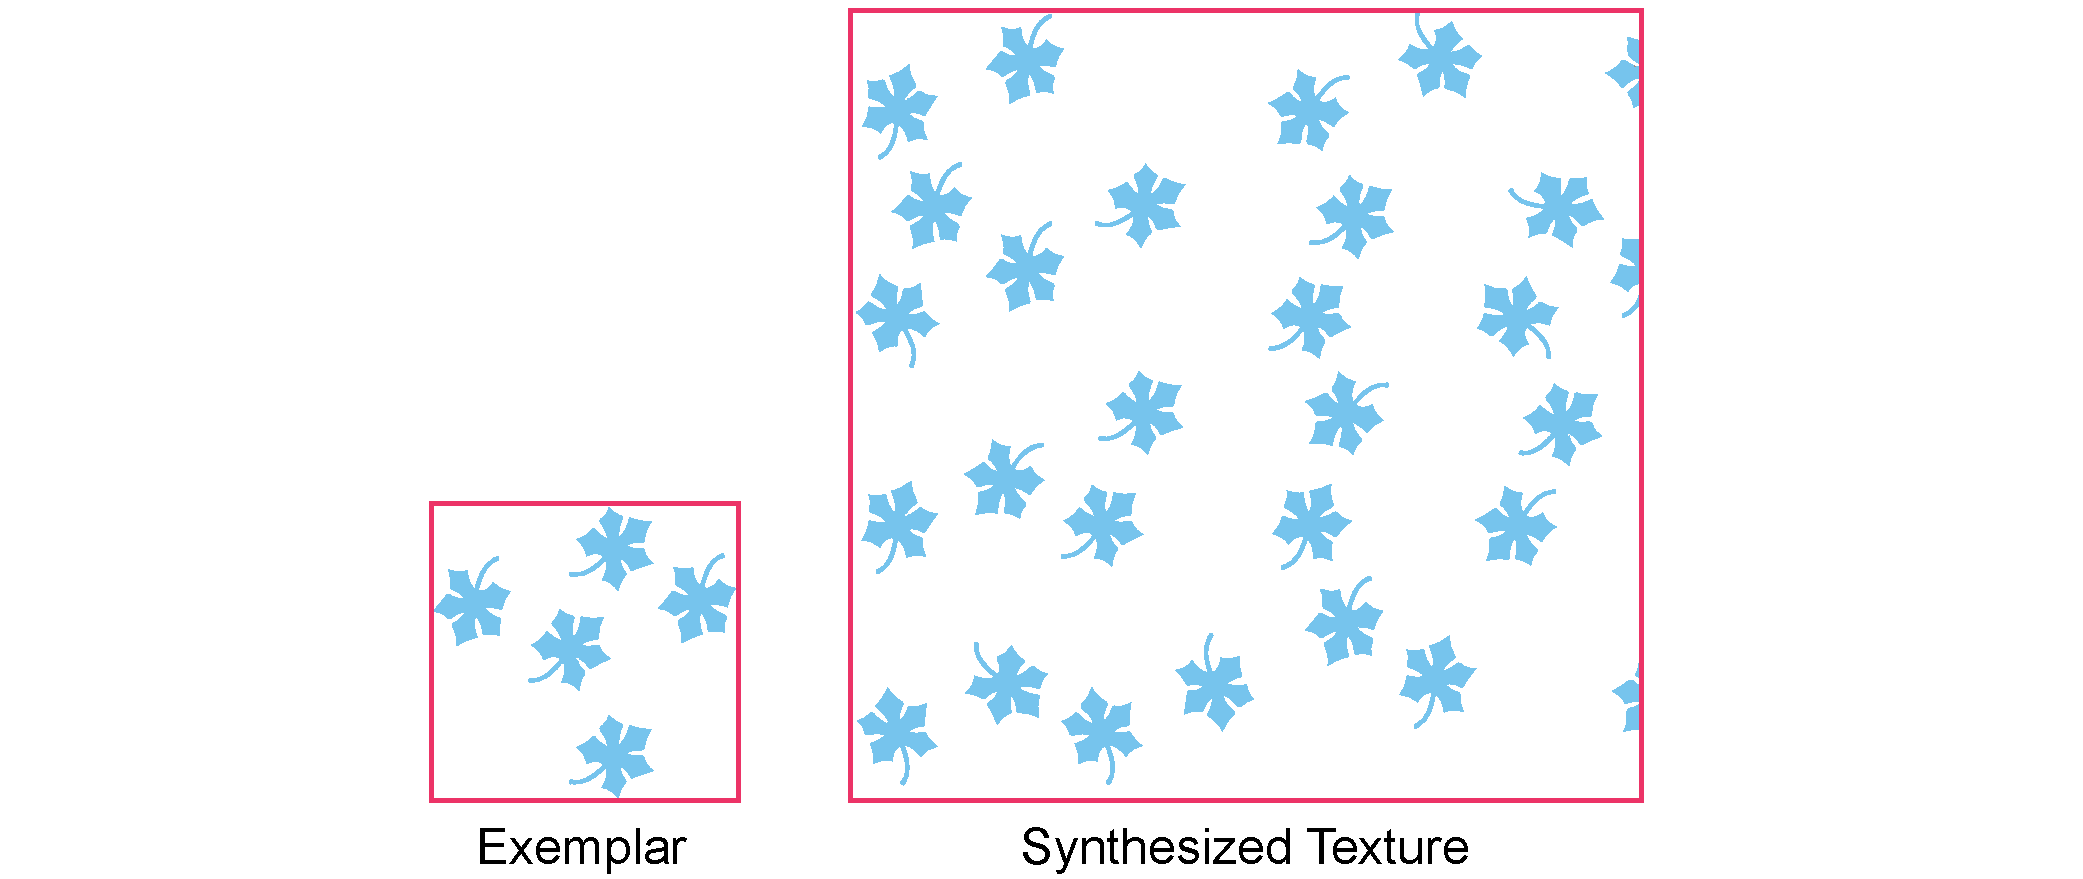
\includegraphics[width=1.0\textwidth]{figures/related/discrete_texture.pdf} 
\caption[A discrete texture]
{\label{fig_discrete_texture} 
\newtext
{
An example of discrete texture synthesis~\cite{AlMeraj2013}.
}
}
\end{figure}



%%%%%%%%%%%%%%%%%%%%%%%%%%%%%%%%%%%%%%%%%%%%%%%%%%%%%%%%%%
\section{3D Packings}
%%%%%%%%%%%%%%%%%%%%%%%%%%%%%%%%%%%%%%%%%%%%%%%%%%%%%%%%%%
\newtext{Collages are arrangements of overlapping elements, similar to
portrait paintings by Giuseppe Arcimboldo.
Gal et al.~\cite{Gal2007B} presented a method for constructing 3D
collages (Figure~\ref{fig_related_gal_ma_chen}a).  
They filled a 3D container with overlapping 3D elements using a greedy
approach and a partial shape matching algorithm.}
\nnewtext{
Similar to the work of Gal et al., Theobalt et al.~\cite{Theobalt2007}
developed a method to generate animated 3D collages, which we will discuss more in Chapter~\ref{chapter_animationpak}.}
\newtext{Huang et al.~\cite{Huang2014} designed a method
to generate mechanical collages, such as giant robots.
All these collage methods require a 3D shape database.} %so they are considered as data-driven. 
%Both these collage methods require a 3D shape database so they can be considered as data-driven. 


\newtext
{
The cutting and packing problem (C\&P) is defined as cutting a large object into smaller parts 
which are then packed inside a container.
C\&P is popular in manufacturing and 3D printing because
objects can be produced with less waste material and packed into a smaller box.
A good cutting process is critical in C\&P, if it can decompose the input object
into simpler parts, then the packing process can be easier.
Chernov et al.~\cite{Chernov2010} proposed a method to decompose a large object
into smaller ``phi objects'' that can be packed more efficiently.
A phi object is defined as a shape whose surface boundaries 
are flat, spherical, cylindrical, or conical.
Vanek et al.~\cite{Vanek2014} introduced PackMerger,
a method to pack thin shells which can be assembled together into
a larger watertight object.
In follow up work, Chen et al.~\cite{Chen2015} introduced Dapper,
a method to cut and pack volumetric printed objects.
}

\newtext
{
In engineering, packings are useful for a number of applications, 
such as product packaging, circuit designs, or mechanical layouts.
This requires elements to be packed without any overlap.
Cagan et al.~\cite{Cagan2002} compiled a survey of 3D packing approaches such as
gradient methods, simulated annealing, and genetic algorithms.
Byholm et al.~\cite{Byholm2009} developed a method
to pack voxelized elements, which are computationally easier for collision detection.
Ma et al.~\cite{Ma2018} proposed a heuristic method to pack non-overlapping triangular meshes 
(Figure~\ref{fig_related_gal_ma_chen}b).
}



%%%%%%%%%%%%%%%%%%%%%%%%%%%%%%%%%%%%%%%%%%%%%%%%%%%%%%%%%%
\section{Packings on Surfaces}
%%%%%%%%%%%%%%%%%%%%%%%%%%%%%%%%%%%%%%%%%%%%%%%%%%%%%%%%%%

Some recent work has explored the elaboration of ornamental
patterns on surfaces, under constraints imposed by fabrication, such as connectivity.  
Chen et al.~\cite{Chen2016} developed a method to generate a filigree pattern,
which is an arrangement of decorative thin rod elements on a surface.
Given an initial random configuration of overlapping elements, their method
removes overlaps by either deforming or trimming the rods.
In similar work, Zehnder et al.~\cite{Zehnder2016} 
proposed a semi-automated tool for deforming ornamental curves to cover a surface, one example is shown in 
Figure~\ref{fig_related_gal_ma_chen}c. 
They started with an \nnewtext{initial, overlap free} configuration of scaled down elements. 
They later grew the elements and avoided overlaps using curve deformation.
Chen et al.~\cite{Chen2017} generated modular surfaces by
computing contact point networks of rigid elements, which can be seen in Figure~\ref{fig_related_gal_ma_chen}d.
Bian et al.~\cite{Bian2018} used Wang tiles made of element parts to generate filigree patterns.
Mart\'{\i}nez et al.~\cite{Martinez2019} developed a CVD-based method to generate
star-shaped tiling patterns that are printed onto tracery sheets.
Their method works by constructing a star-shaped metric to manipulate the Voronoi cell shapes. 

%\begin{figure}
%\centering
%\includegraphics[width=1.0\textwidth]{figures/related/arcimboldo_gal.pdf} 
%\caption[Examples of 3D packing arrangements]
%{\label{fig_related_arcimboldo_gal} 
%\newtext
%{
%3D packing arrangements:
%(Left) Vertumnus painting by Giuseppe Arcimboldo (Skokloster Castle, Skokloster, Sweden). 
%(Right) An Arcimboldo-like 3D packing~\cite{Gal2007B}.
%}
%}
%\end{figure}

%\makeatletter % brooo
%\setlength{\@fptop}{0pt} % brooo
%\makeatother % brooo
%\begin{figure}
%\centering
%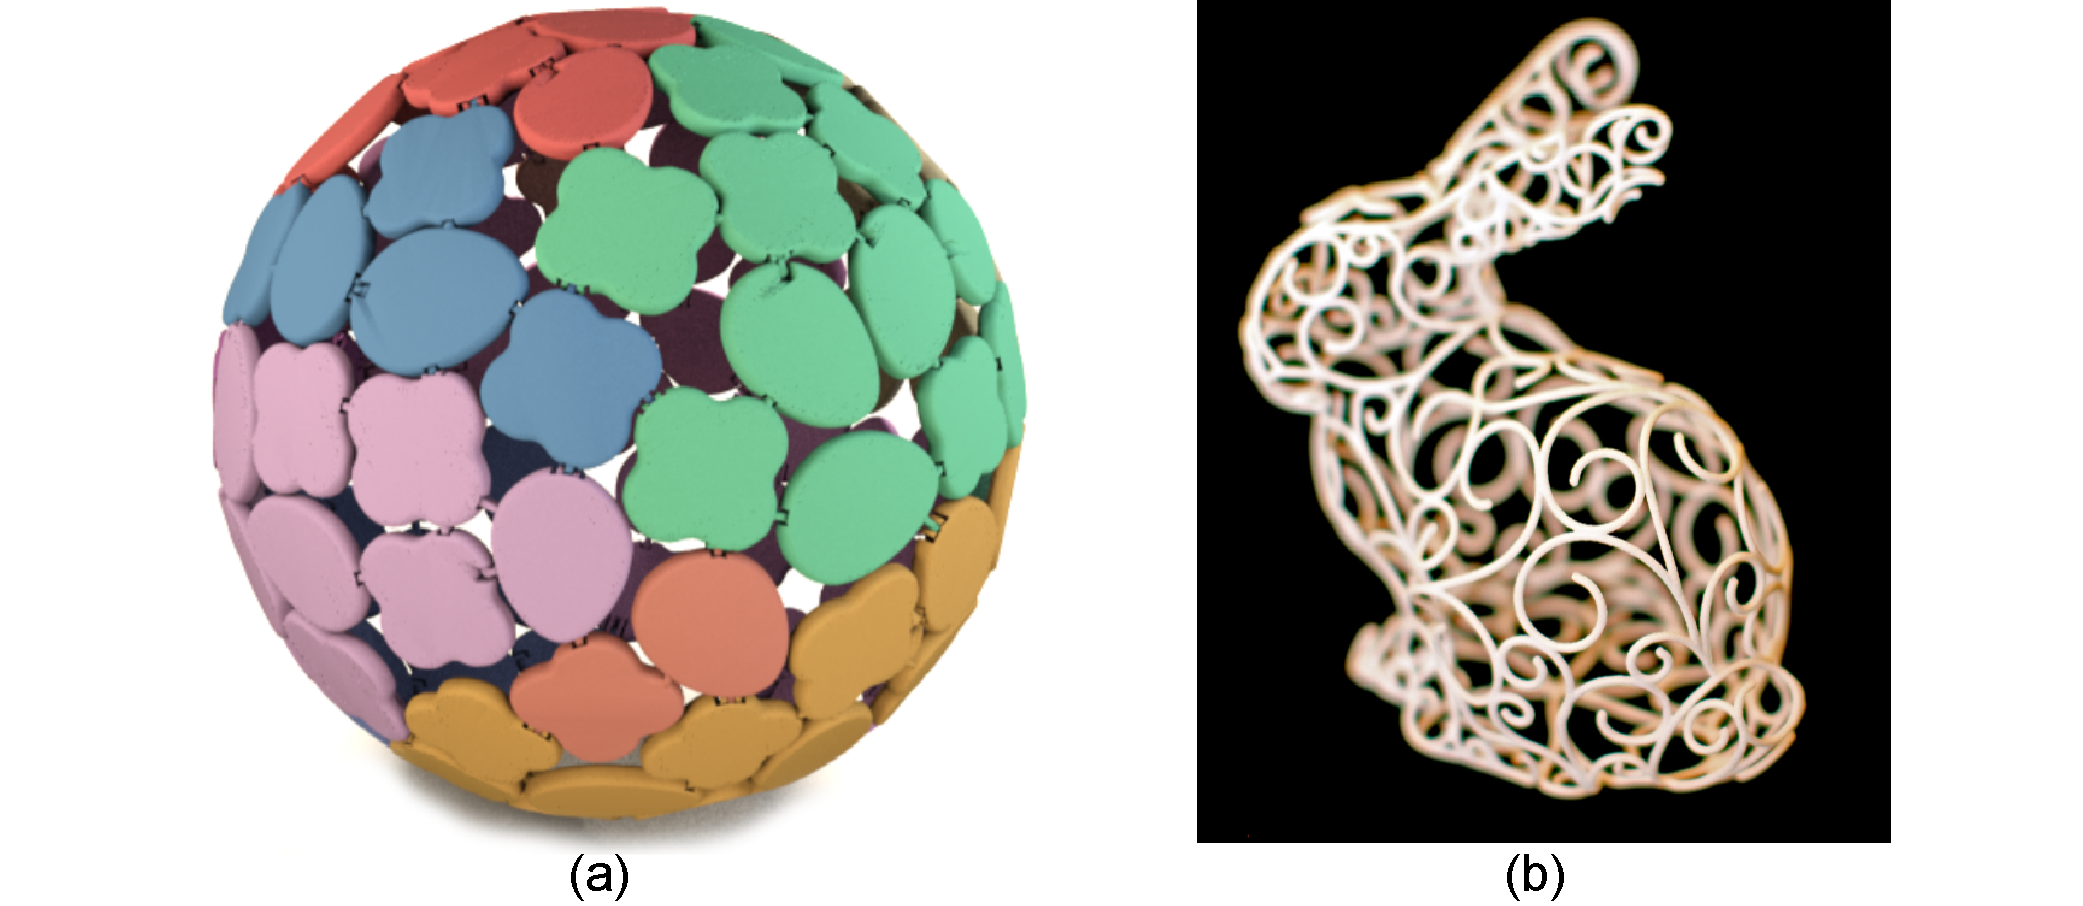
\includegraphics[width=1.0\textwidth]{figures/related/chen_zehnder.pdf} 
%\caption[Two example of packings on surfaces]
%{\label{fig_related_chen_zehnder} 
%\nnewtext
%{
%Two example of packings on surfaces:
%(a) Elements packed on a surface and connected by hinges~\cite{Chen2017}.
%(b) Curve elements arranged on a bunny surface~\cite{Zehnder2016}.
%}
%}
%\end{figure}

%\makeatletter % brooo
%\setlength{\@fptop}{0pt} % brooo
%\makeatother % brooo
\begin{figure}
\centering
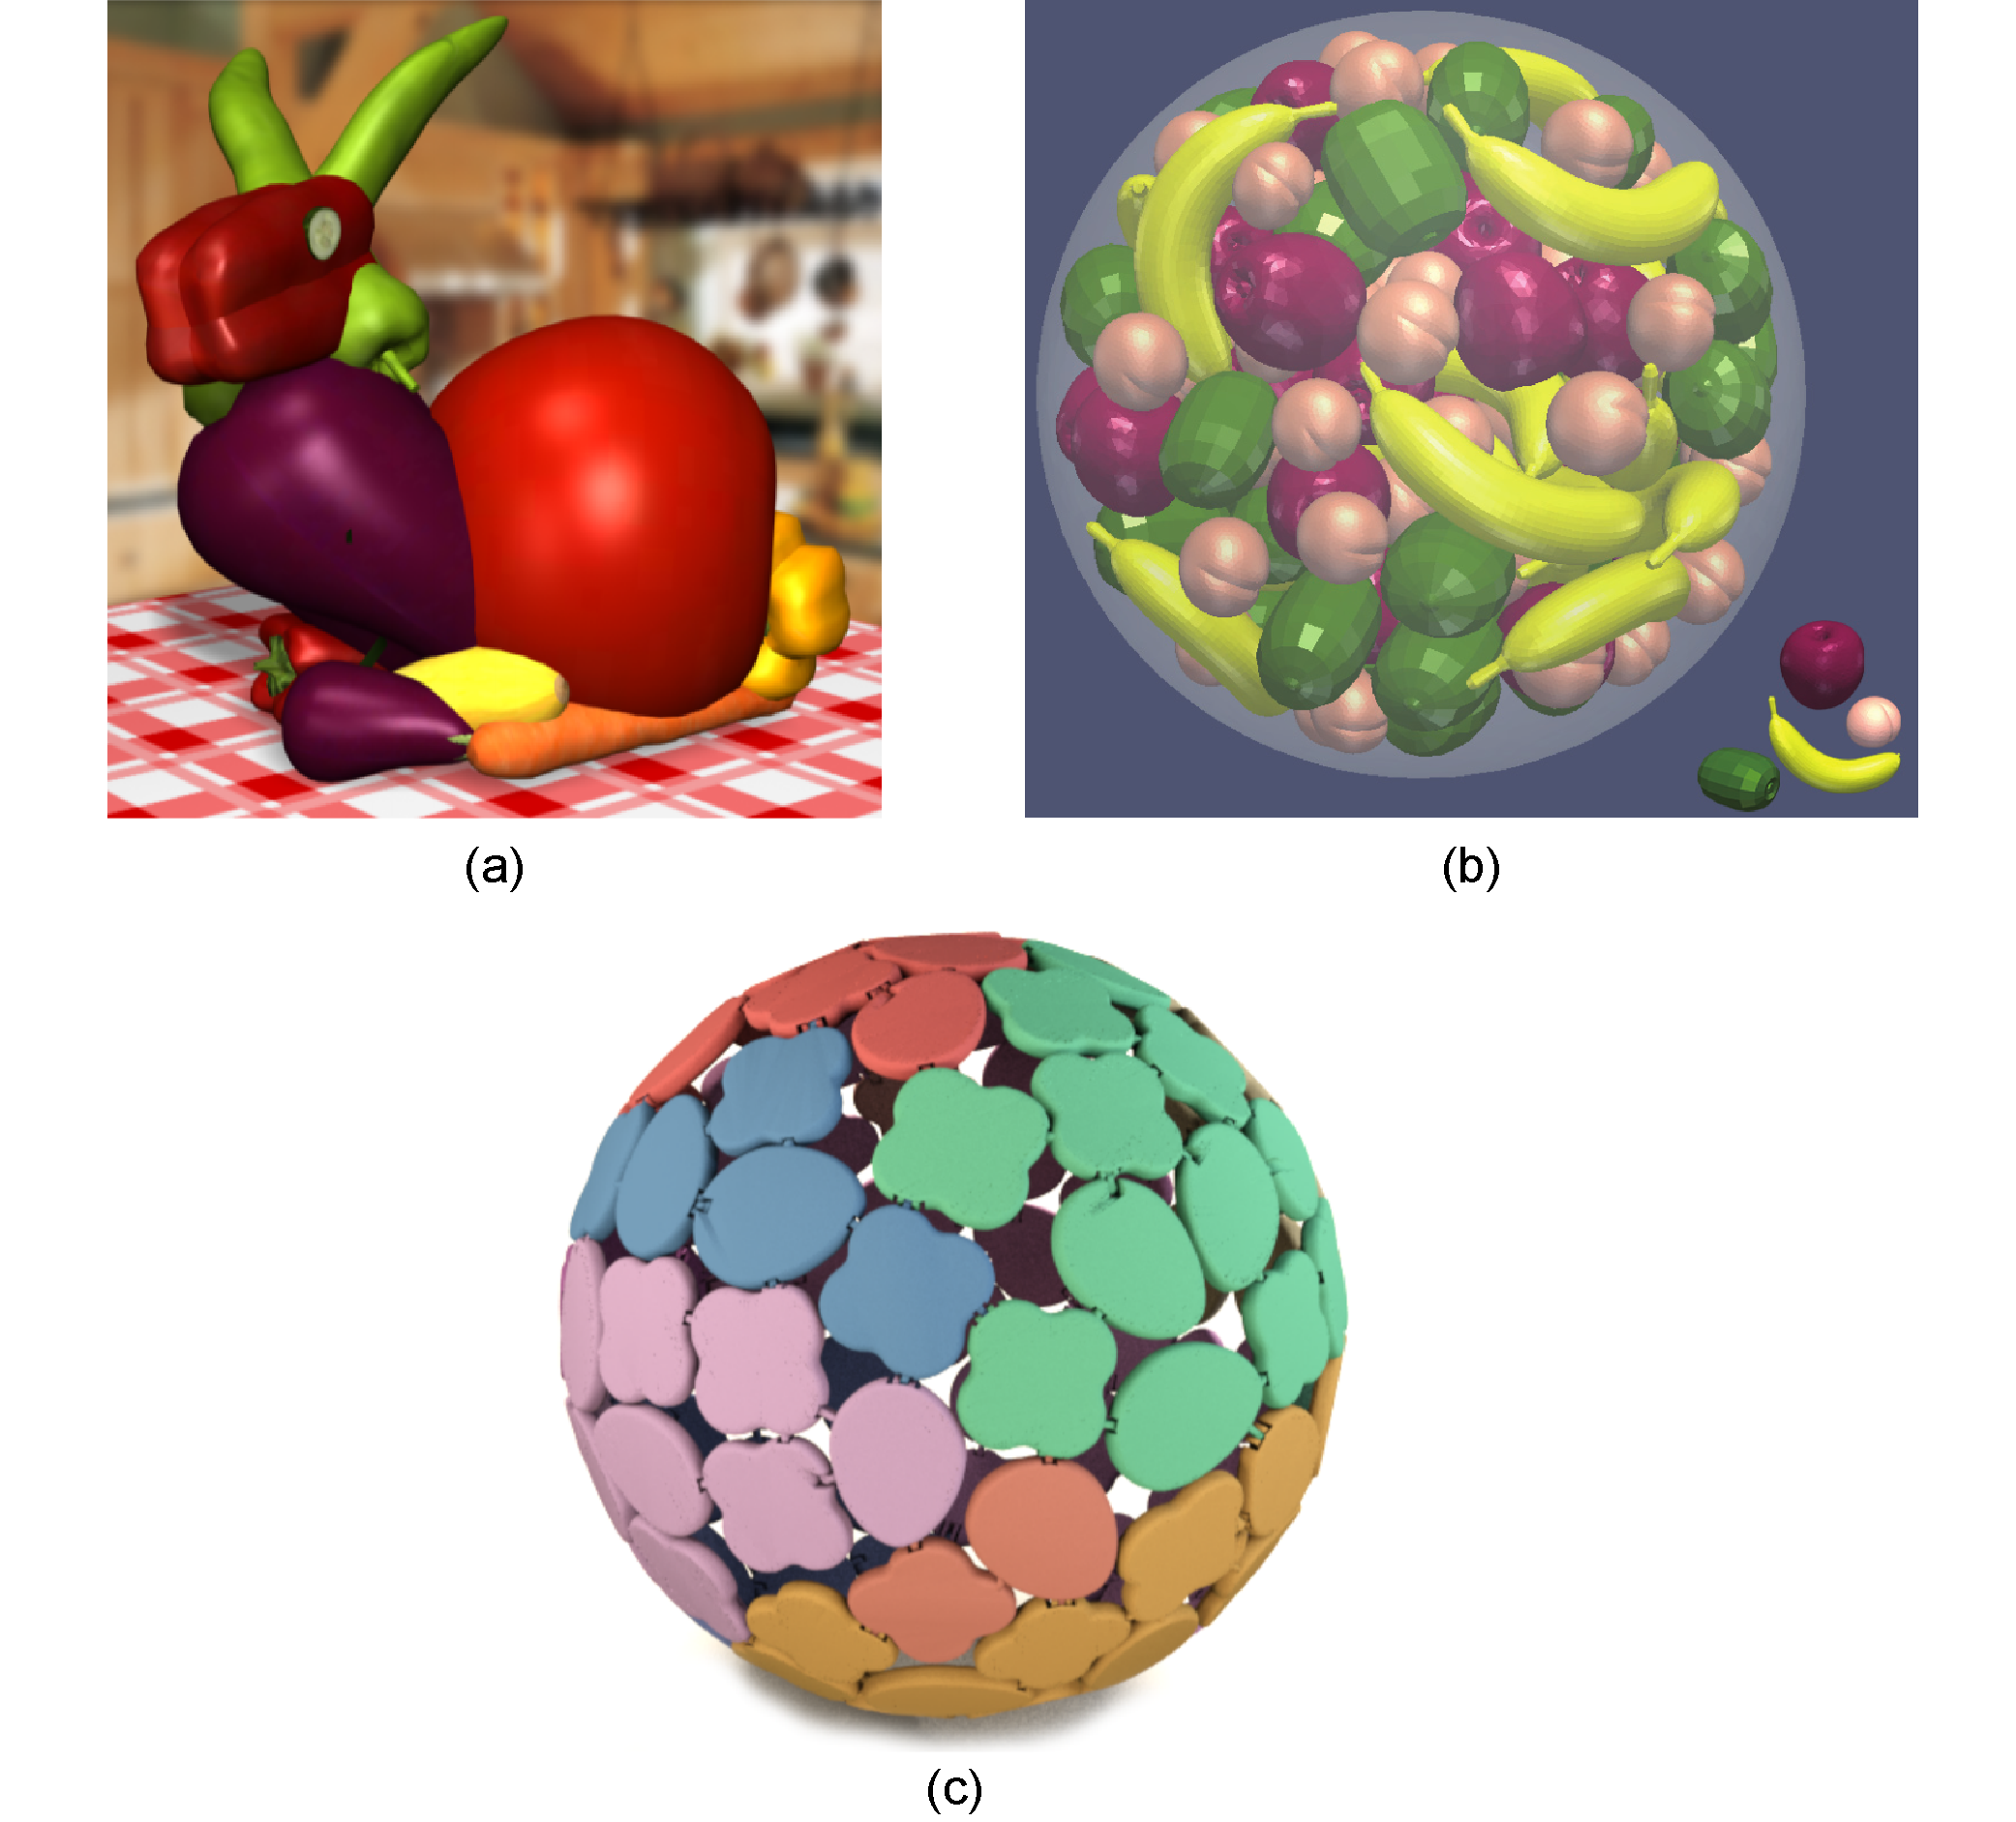
\includegraphics[width=1.0\textwidth]{figures/related/gal_ma_chen.pdf} 
\caption[Examples of 3D packings and packings on surfaces]
{\label{fig_related_gal_ma_chen} 
\nnewtext
{
Examples of 3D packings and packings on surfaces.
(a) An Arcimboldo-like packing of overlapping 3D elements~\cite{Gal2007B}. 
(c) A packing of non-overlapping 3D elements~\cite{Ma2018}.
(c) Deformed curve selements that fill a surface~\cite{Zehnder2016}.
(d) Elements that fill a surface which are connected by hinges~\cite{Chen2017}.
}
}
\end{figure}

